This chapter presents a comparison of Run 2 ICARUS data and the corresponding expectations from simulation. Section \ref{sec:run2_dataset} describes the dataset used for this analysis, including the rejection of subsets of the dataset due to non-ideal detector conditions and the steps taken to comply with the ICARUS blinding policy. Section \ref{sec:data_comparisons} presents the comparison of data and simulation in each of the reconstructed variables along with some discussion on the observed data/simulation agreement. 


\subsection{Run 2 Dataset}
\label{sec:run2_dataset}

The dataset used for this analysis consists of the ICARUS Run 2 data collected between December 20, 2022 and July 16, 2023. This period of data collection represents the largest dataset with stable detector conditions collected by the ICARUS T600 detector at Fermilab to date, corresponding to approximately $2.05 \times 10^{20}$ POT.

\subsubsection{Data Quality}
\label{sec:data_quality}

Though the detector was overall stable throughout the duration of this physics run, there were instances of detector instabilities that resulted in portions of DAQ runs being flagged as bad. These instabilities were typically due to single-component failures, such as the power supply of a TPC readout crate, or due to issues with the DAQ, trigger, cathode, or wire bias systems. These issues were logged and used as part of the data processing to identify and remove bad runs from the dataset. This results in a final dataset of around $1.92 \times 10^{20}$ POT.

\subsubsection{The ICARUS Blinding Policy}
\label{sec:blinding_policy}

The ICARUS collaboration has an official data blinding policy in place to prevent experimenter bias in the analysis of the data. The philosophy behind this policy is to ensure that an analyzer will not prematurely access the data in a statistically significant way that could influence the development of the analysis. By default, only $10\%$ of the data is fully unblinded for the purpose of developing the analysis, while the remaining $90\%$ is kept blinded until the analysis is finalized. The blinding policy also sets a process for accessing the blinded data, which is typically done in stages following the submission of technical documentation of the analysis and review by the collaboration. 

In practical terms, this policy is enforced at the level of the ICARUS data processing and analysis software. A decision is made per-event to determine if the event is blinded or unblinded using a random number service that is seeded with a configurable parameter. This allows for reproducible blinding decisions, which is important for maintaining the same set of blinded events across all data-processing campaigns. The files (``Common Analysis Framework'' files, or CAF files) containing analysis-level information for the $10\%$ of the data that is declared unblinded are kept entirely separate from the CAF files containing the blinded data. It is worth noting that this policy only applies to data streams that contain neutrino interactions and not to cosmic-only data streams such as the off-beam data.

The goals of this analysis are to demonstrate the performance of the ICARUS machine-learning analysis chain on the Run 2 dataset in signal channels of relevance for ICARUS and the SBN Program. This can be done with the $10\%$ of the data that is unblinded and does not require the increased statistics of the full Run 2 dataset. The final dataset size for this analysis is therefore $1.92 \times 10^{19}$ POT, after accounting for data processing inefficiencies and removing data from periods of detector instability. The data used for this analysis was processed in full compliance with the ICARUS blinding policy. At no point during the development of this analysis was any portion of the blinded data accessed. 

\subsection{Data/Simulation Comparisons}
\label{sec:data_comparisons}
This section presents the comparison of Run 2 ICARUS data and the corresponding expectations from simulation across a wide range of variables. The comparison is performed for the three signal channels of interest for ICARUS and the SBN Program: $\mathrm{1\mu 1p}$, $\mathrm{1\mu Np}$, and $\nu_\mu$ CC inclusive. Agreement between data and simulation is crucial for demonstrating the readiness of the ICARUS machine-learning analysis chain for future analyses. 

Each of the subsections below shows a set of distributions for a particular set of variables. In each distribution, the data is shown as black points with error bars representing the statistical uncertainty on the data. The expectation from the combination of simulation and off-beam data is shown as the filled histogram, with the error bands representing the full uncertainty as described in Chapter \ref{chap:systematics}. The lower panel of each plot shows the ratio of data to the expectation with the same error bars and bands superimposed.

To quantitatively assess the agreement, the $\chi^2$ test statistic is calculated for each distribution. The $\chi^2$ is calculated using the sum of the overall covariance matrix for the expectation and the statistical covariance matrix for the data:

\begin{equation}
    \chi^2 = \sum_{i,j} \left( O_i - E_i \right) \left( \Sigma^{-1} \right)_{ij} \left( O_j - E_j \right)
\end{equation}

\noindent
where $O_i$ and $E_i$ are the observed and expected values in bin $i$, respectively, and $\Sigma$ is the covariance matrix. The $\chi^2$ is then normalized by the number of degrees of freedom, which is the number of nonzero bins minus one. The $\chi^2$ per degree of freedom is reported for each distribution.

\subsubsection{Comparisons for Interaction Kinematic Variables}
\label{sec:datamc_interaction_kinematic_variables}

\begin{figure}
    \centering
    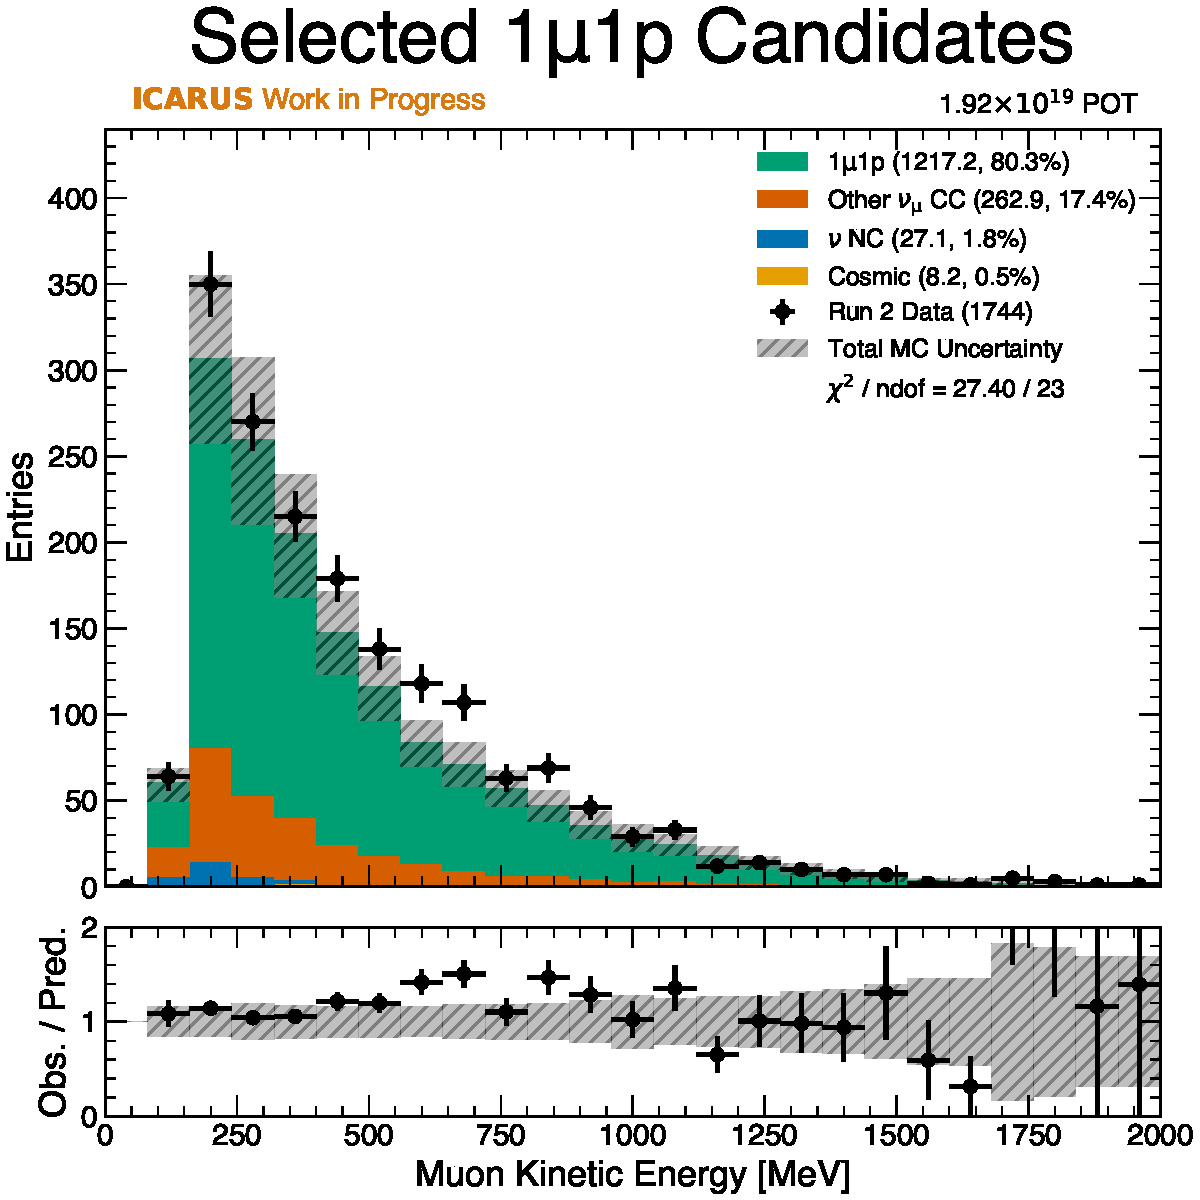
\includegraphics[width=0.42\textwidth]{figures/data_mc_comparisons/datamc_hist1d_1mu1p_muon_ke.pdf}
    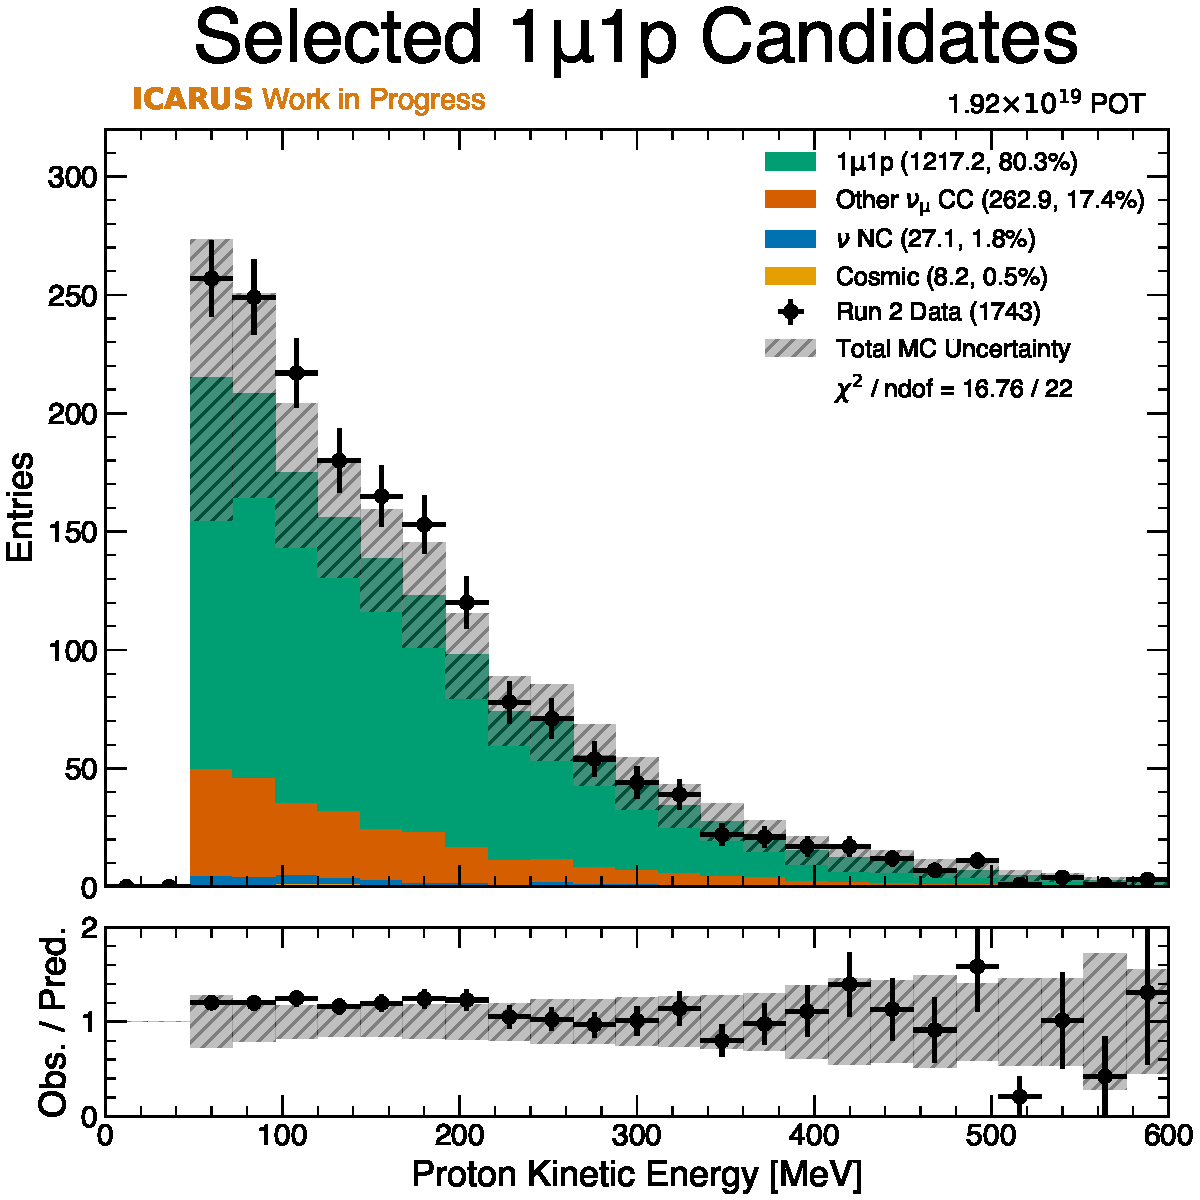
\includegraphics[width=0.42\textwidth]{figures/data_mc_comparisons/datamc_hist1d_1mu1p_proton_ke.pdf}
    \\
    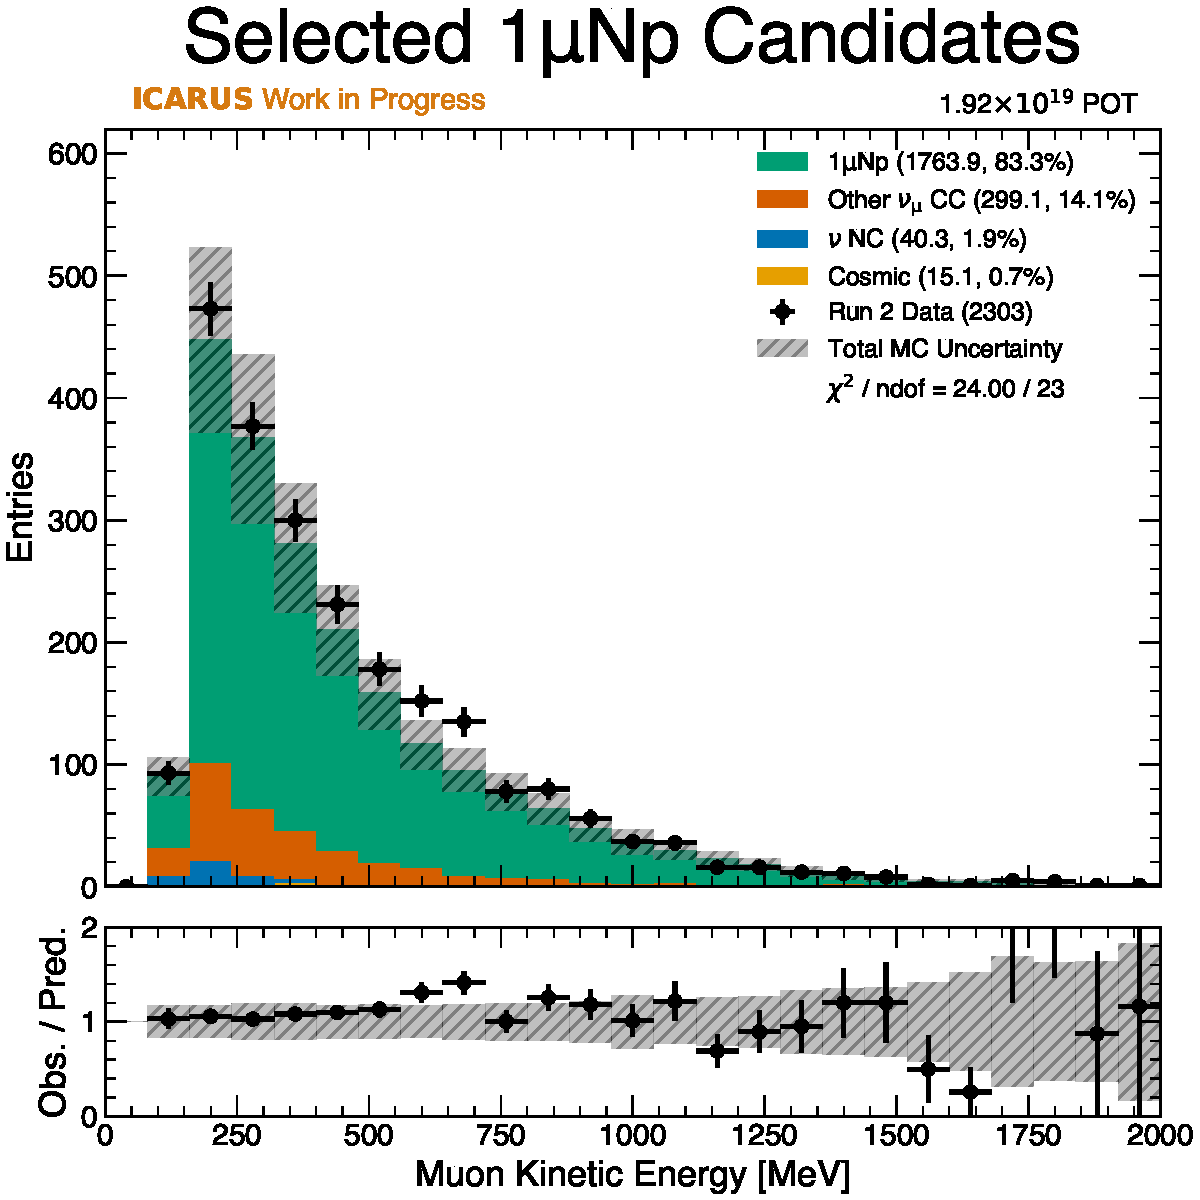
\includegraphics[width=0.42\textwidth]{figures/data_mc_comparisons/datamc_hist1d_1muNp_muon_ke.pdf}
    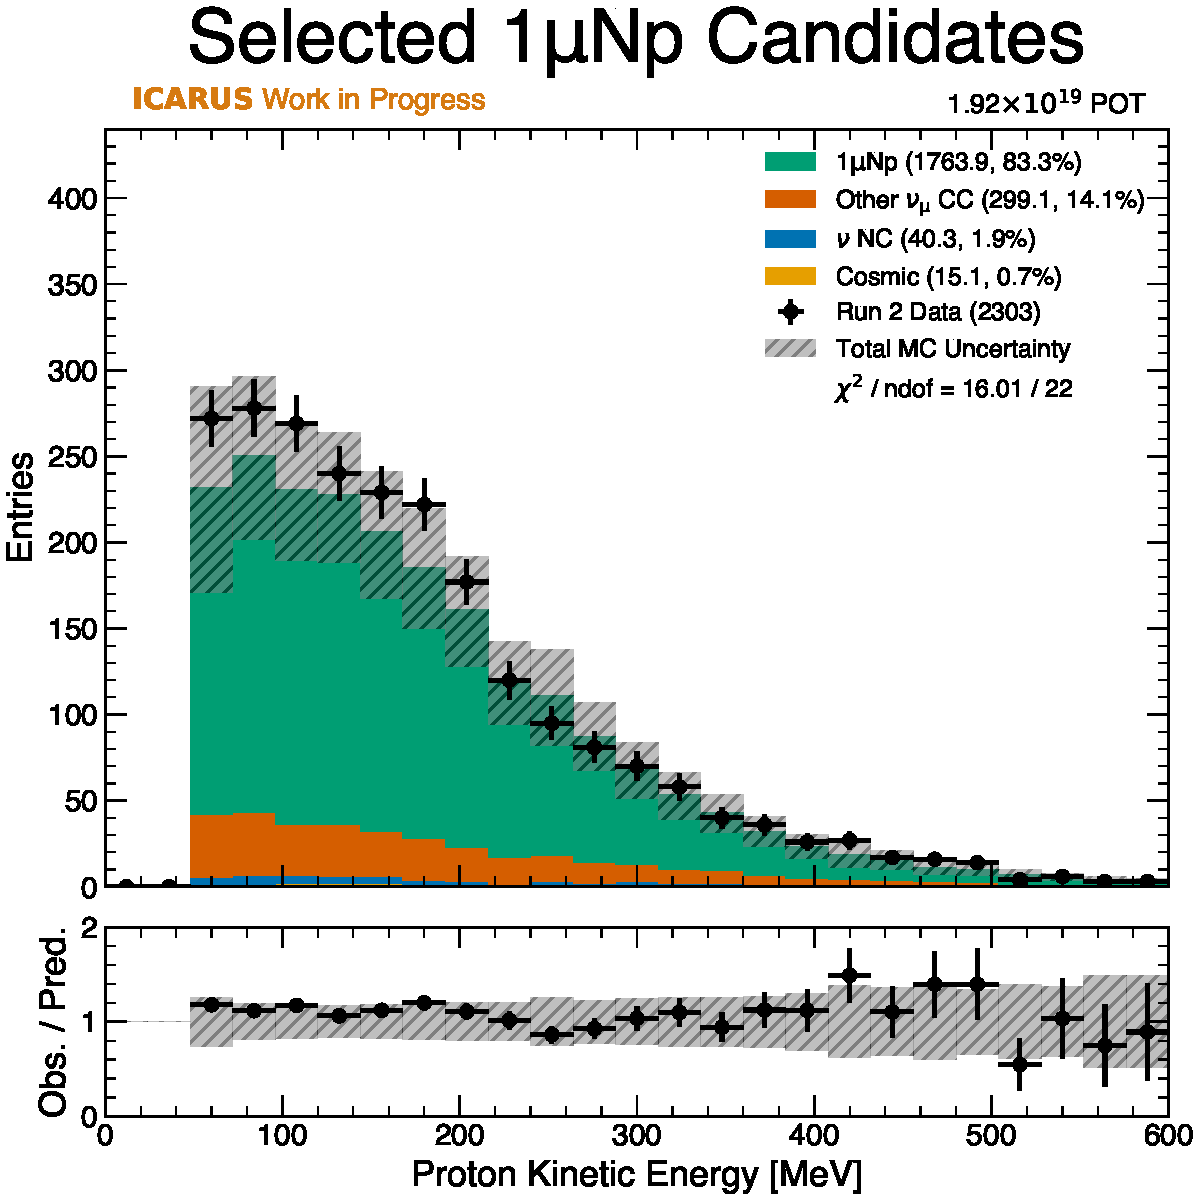
\includegraphics[width=0.42\textwidth]{figures/data_mc_comparisons/datamc_hist1d_1muNp_proton_ke.pdf}
    \\
    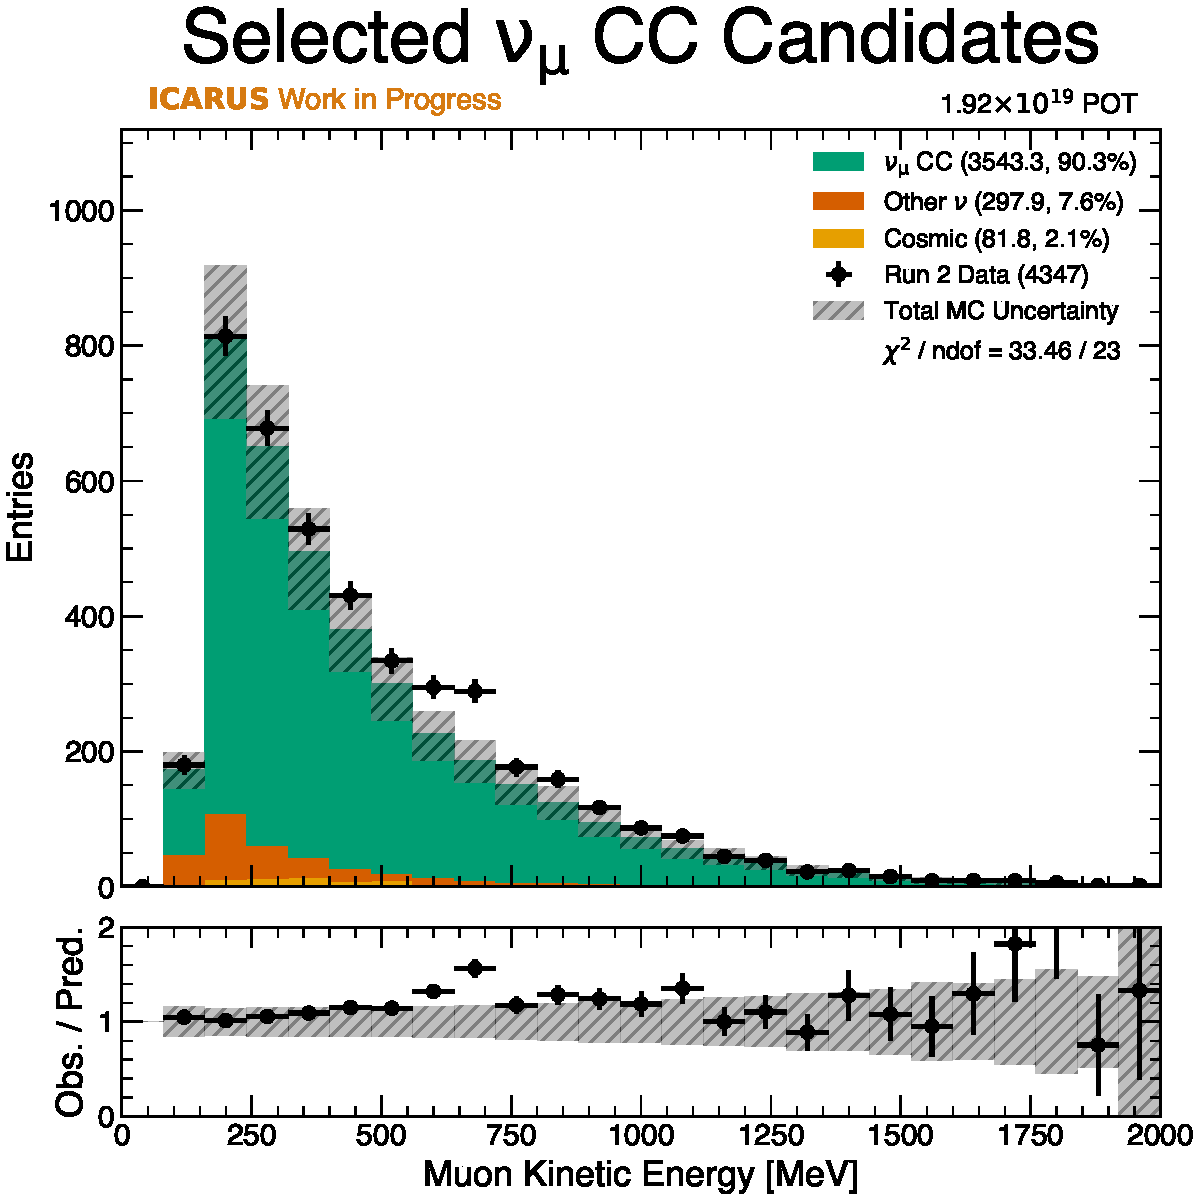
\includegraphics[width=0.42\textwidth]{figures/data_mc_comparisons/datamc_hist1d_1muX_muon_ke.pdf}
    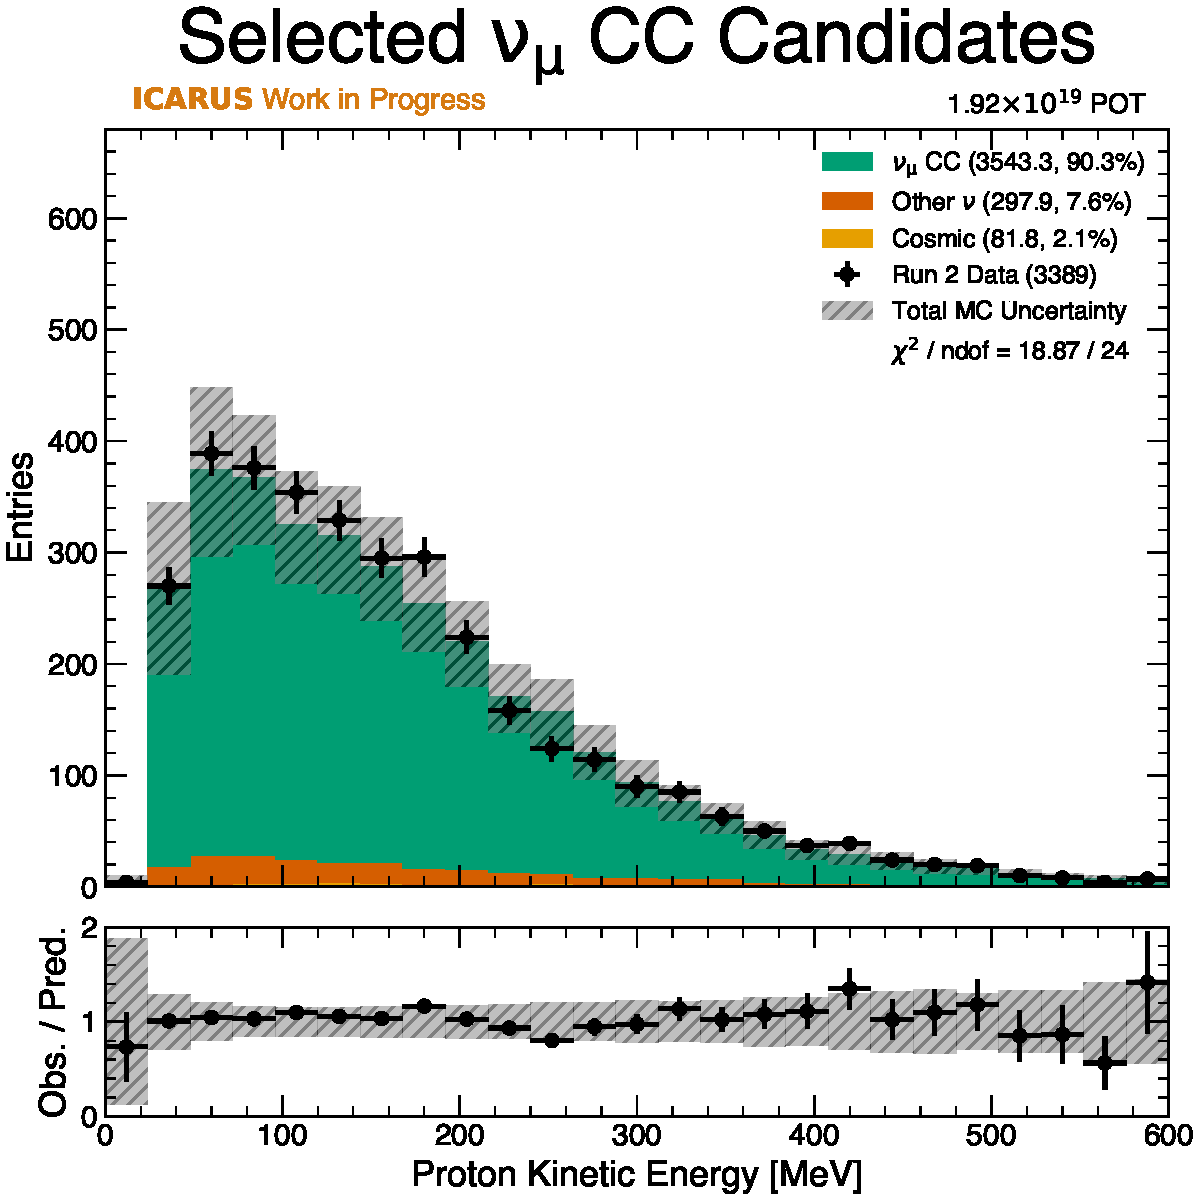
\includegraphics[width=0.42\textwidth]{figures/data_mc_comparisons/datamc_hist1d_1muX_proton_ke.pdf}
    \caption{Comparison of data and simulation for the kinetic energy of the muon (left) and the most energetic proton (right) for each of the three signal channels: from top to bottom $\mathrm{1\mu 1p}$, $\mathrm{1\mu Np}$, and $\nu_\mu$ CC inclusive.}
    \label{fig:datamc_muon_proton_ke}
\end{figure}

\begin{figure}
    \centering
    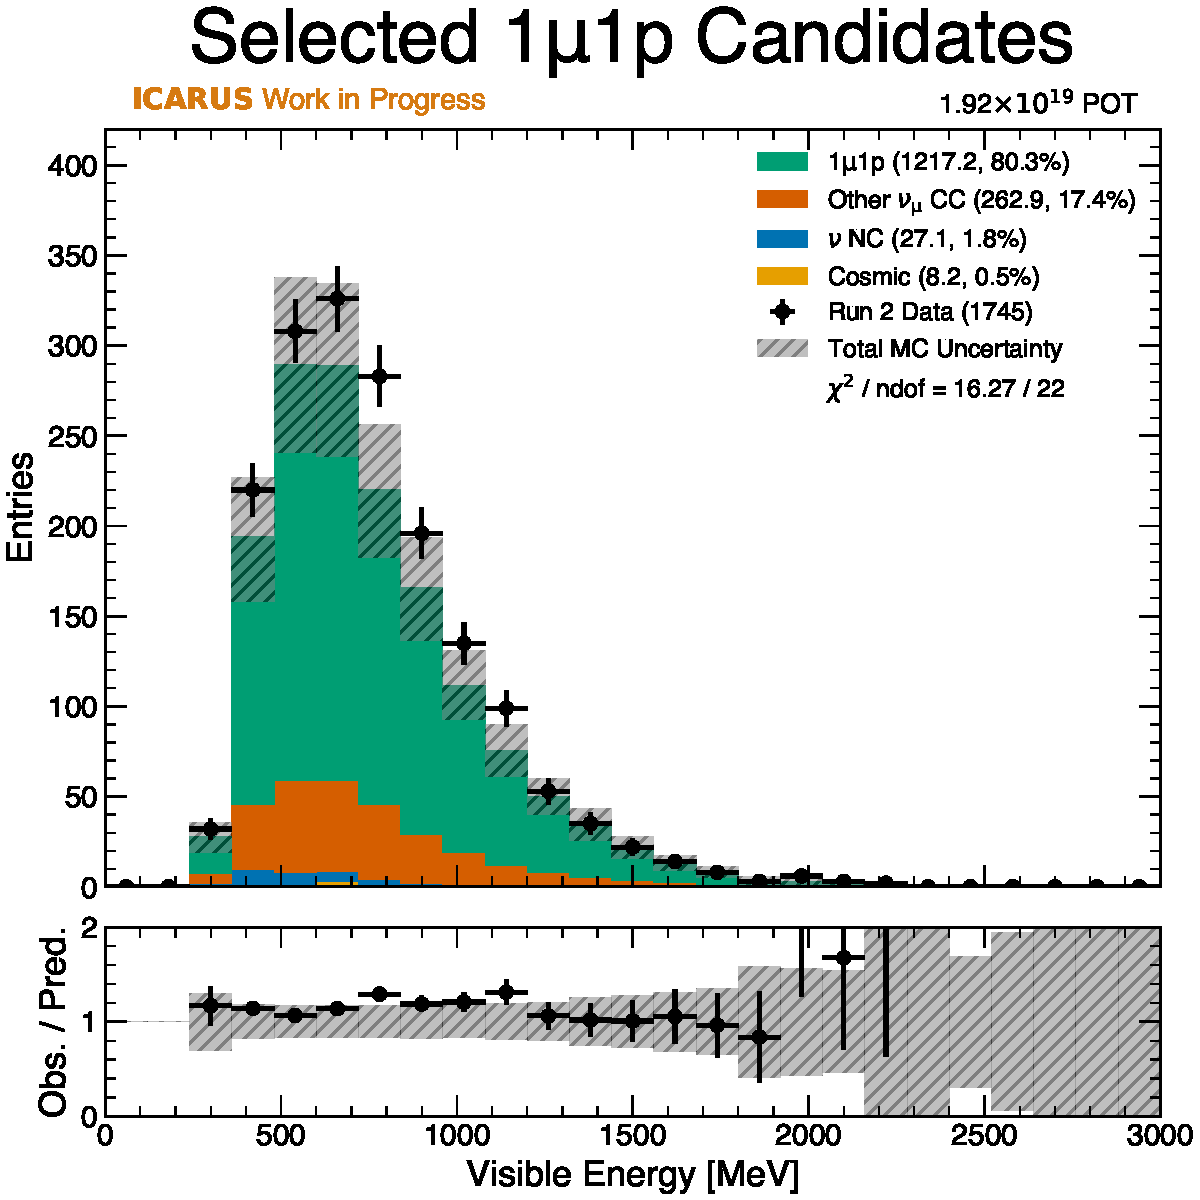
\includegraphics[width=0.42\textwidth]{figures/data_mc_comparisons/datamc_hist1d_1mu1p_visible_energy.pdf}\\
    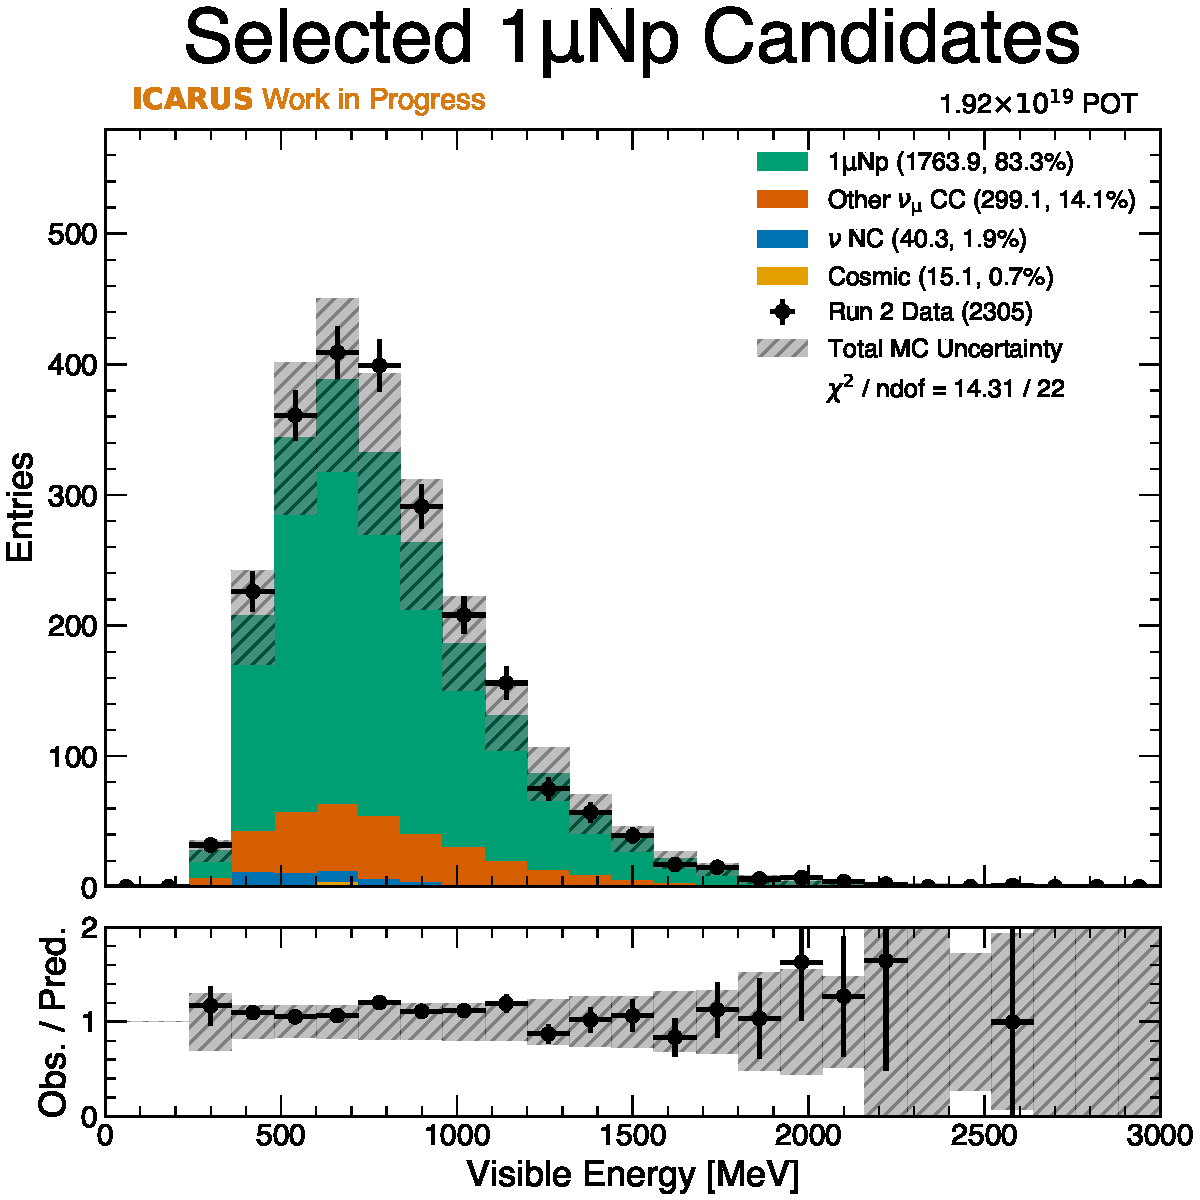
\includegraphics[width=0.42\textwidth]{figures/data_mc_comparisons/datamc_hist1d_1muNp_visible_energy.pdf}\\
    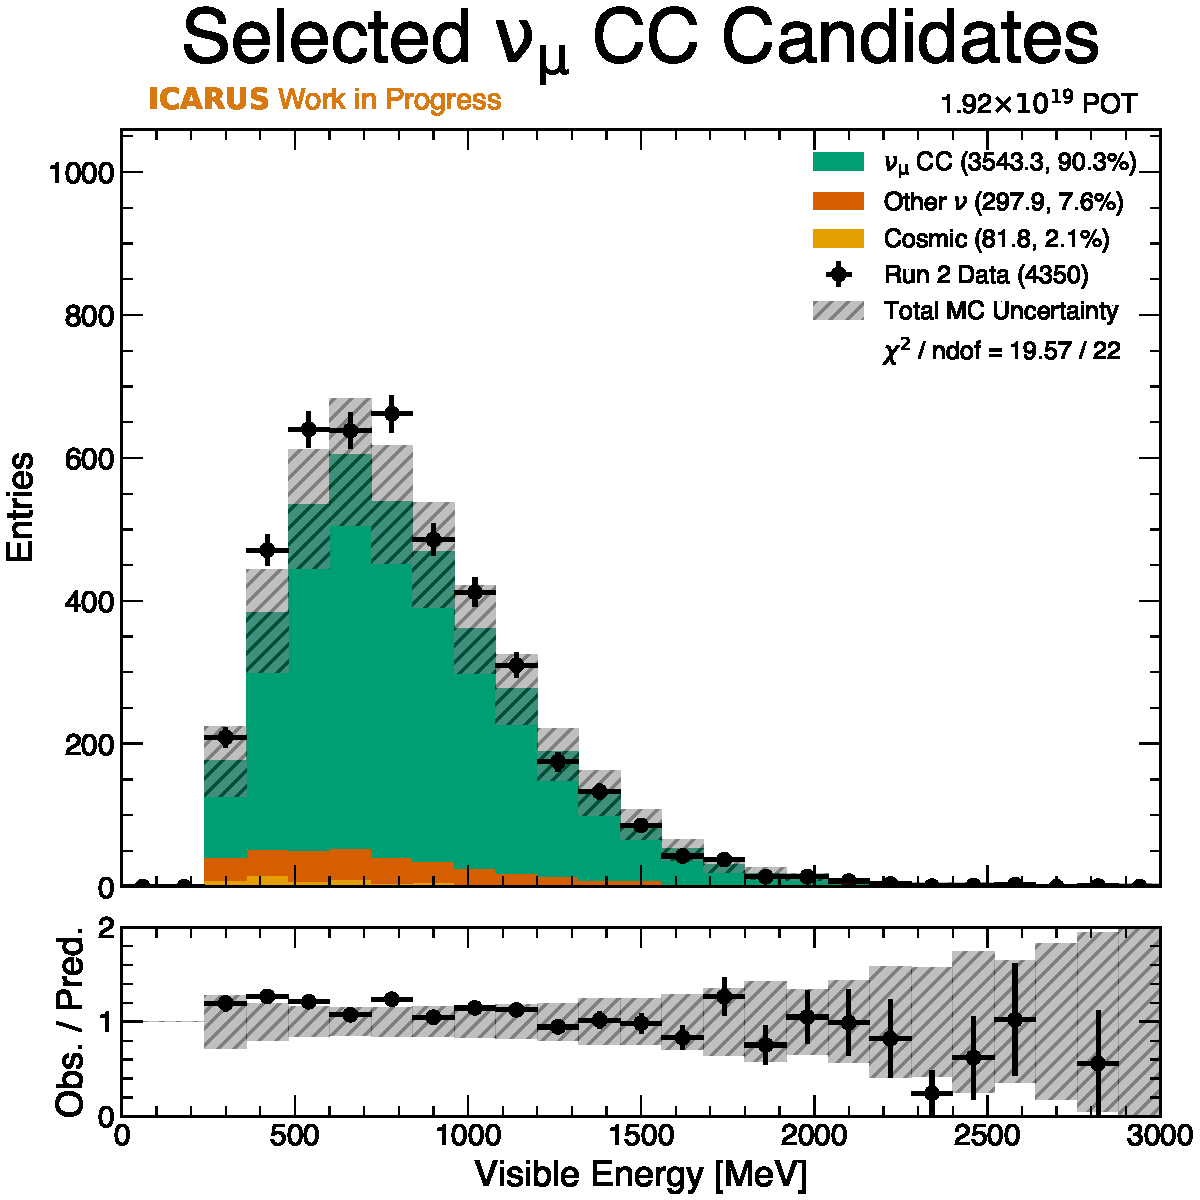
\includegraphics[width=0.42\textwidth]{figures/data_mc_comparisons/datamc_hist1d_1muX_visible_energy.pdf}\\
    \caption{Comparison of data and simulation for the total visible energy of the interaction for each of the signal channels: from top to bottom $\mathrm{1\mu 1p}$, $\mathrm{1\mu Np}$, and $\nu_\mu$ CC inclusive.}
    \label{fig:datamc_visible_energy}
\end{figure}

\begin{figure}
    \centering
    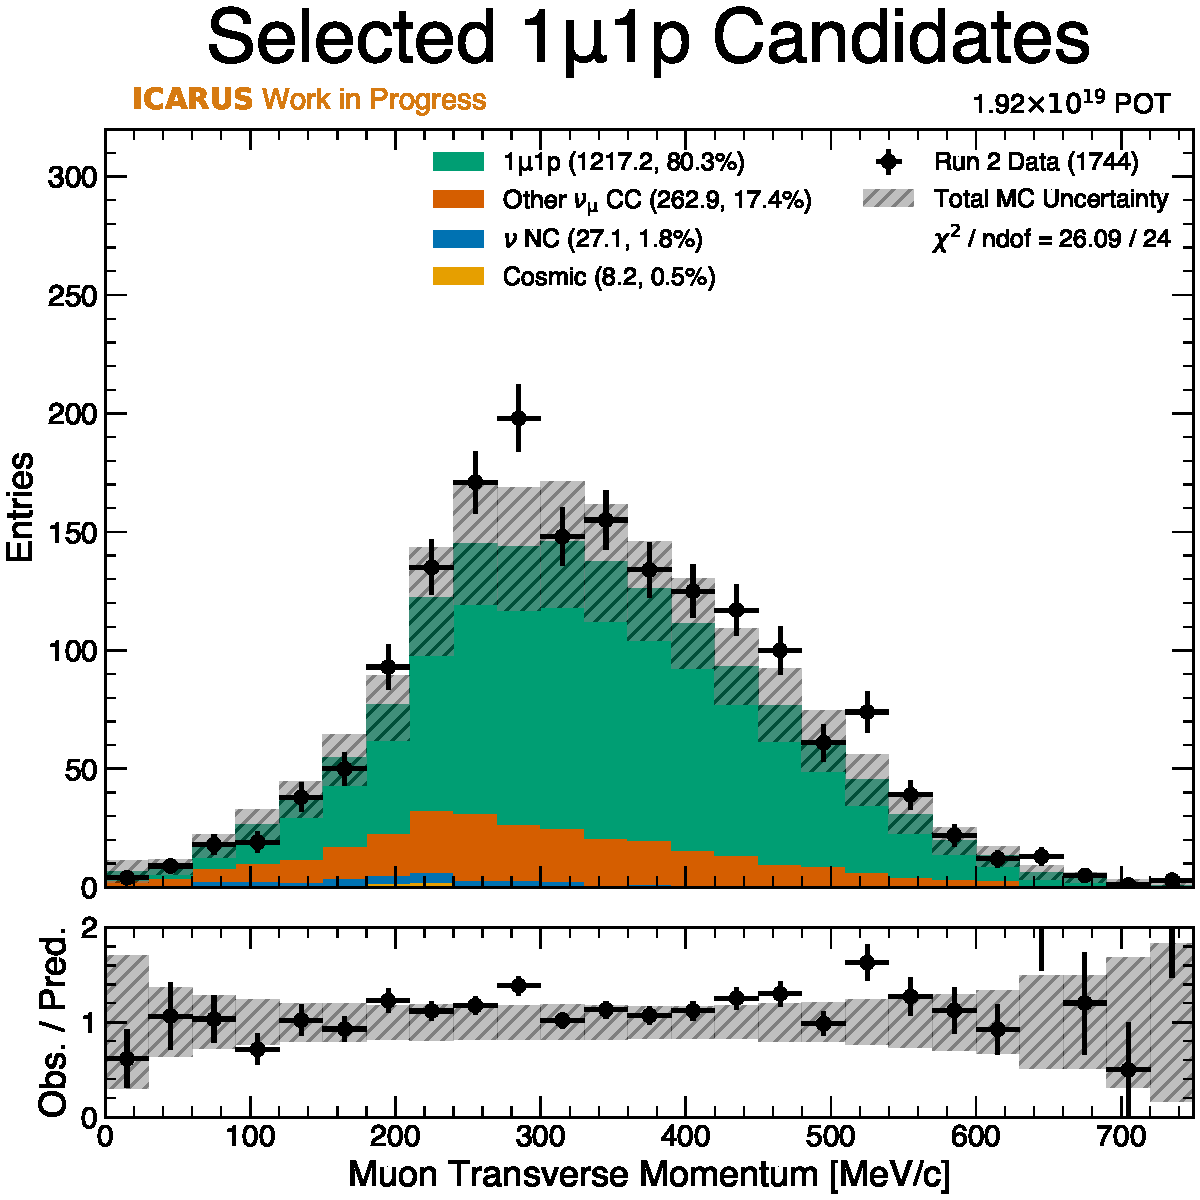
\includegraphics[width=0.41\textwidth]{figures/data_mc_comparisons/datamc_hist1d_1mu1p_muon_pt.pdf}
    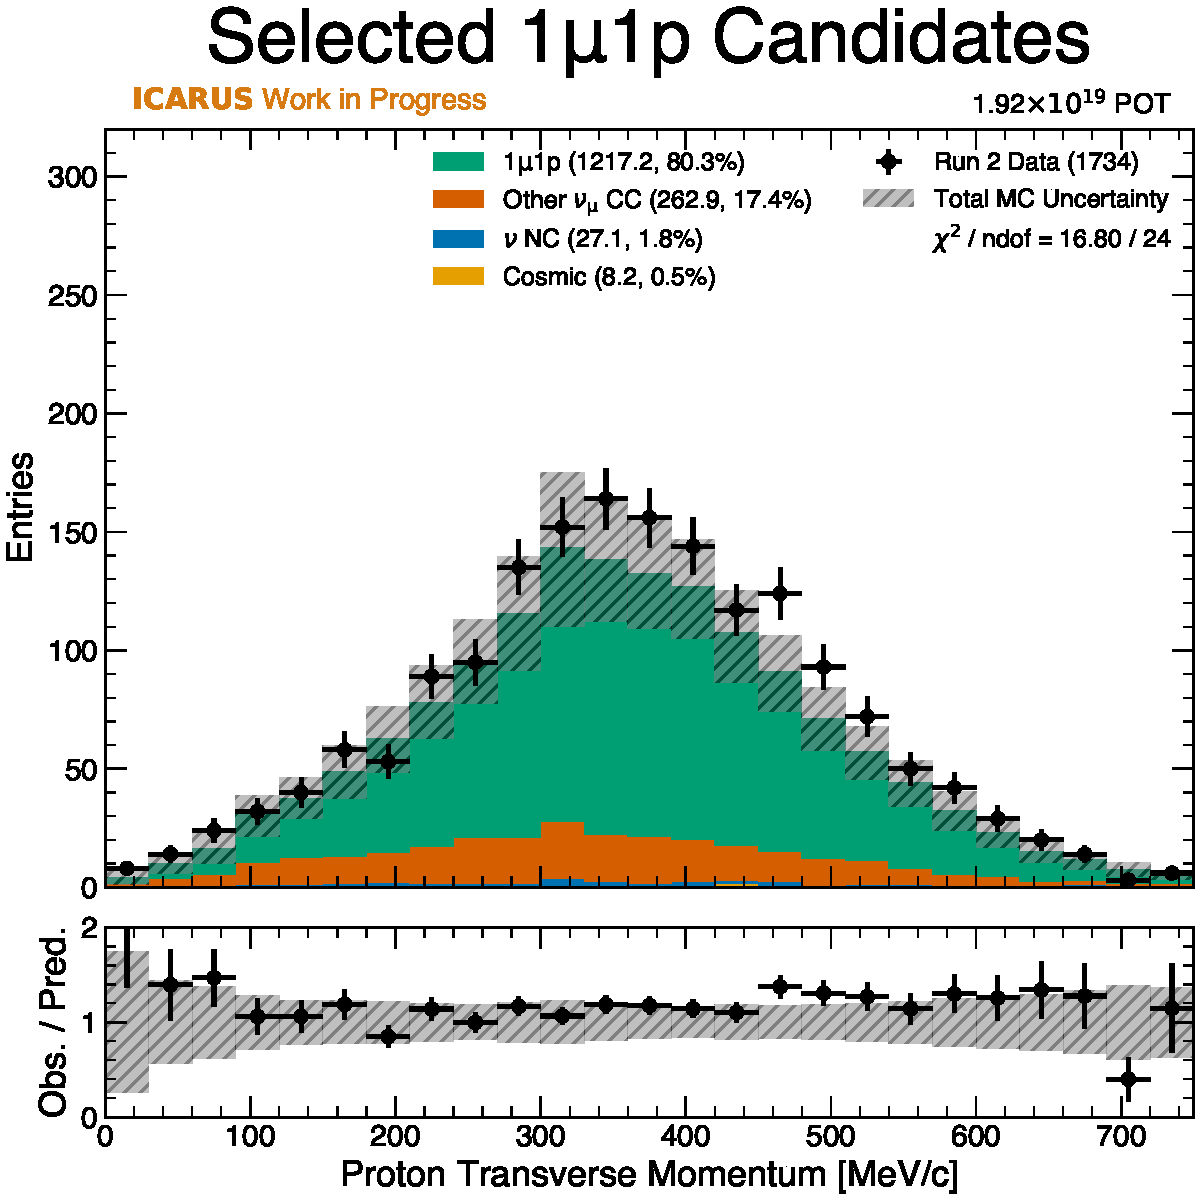
\includegraphics[width=0.41\textwidth]{figures/data_mc_comparisons/datamc_hist1d_1mu1p_proton_pt.pdf}
    \\
    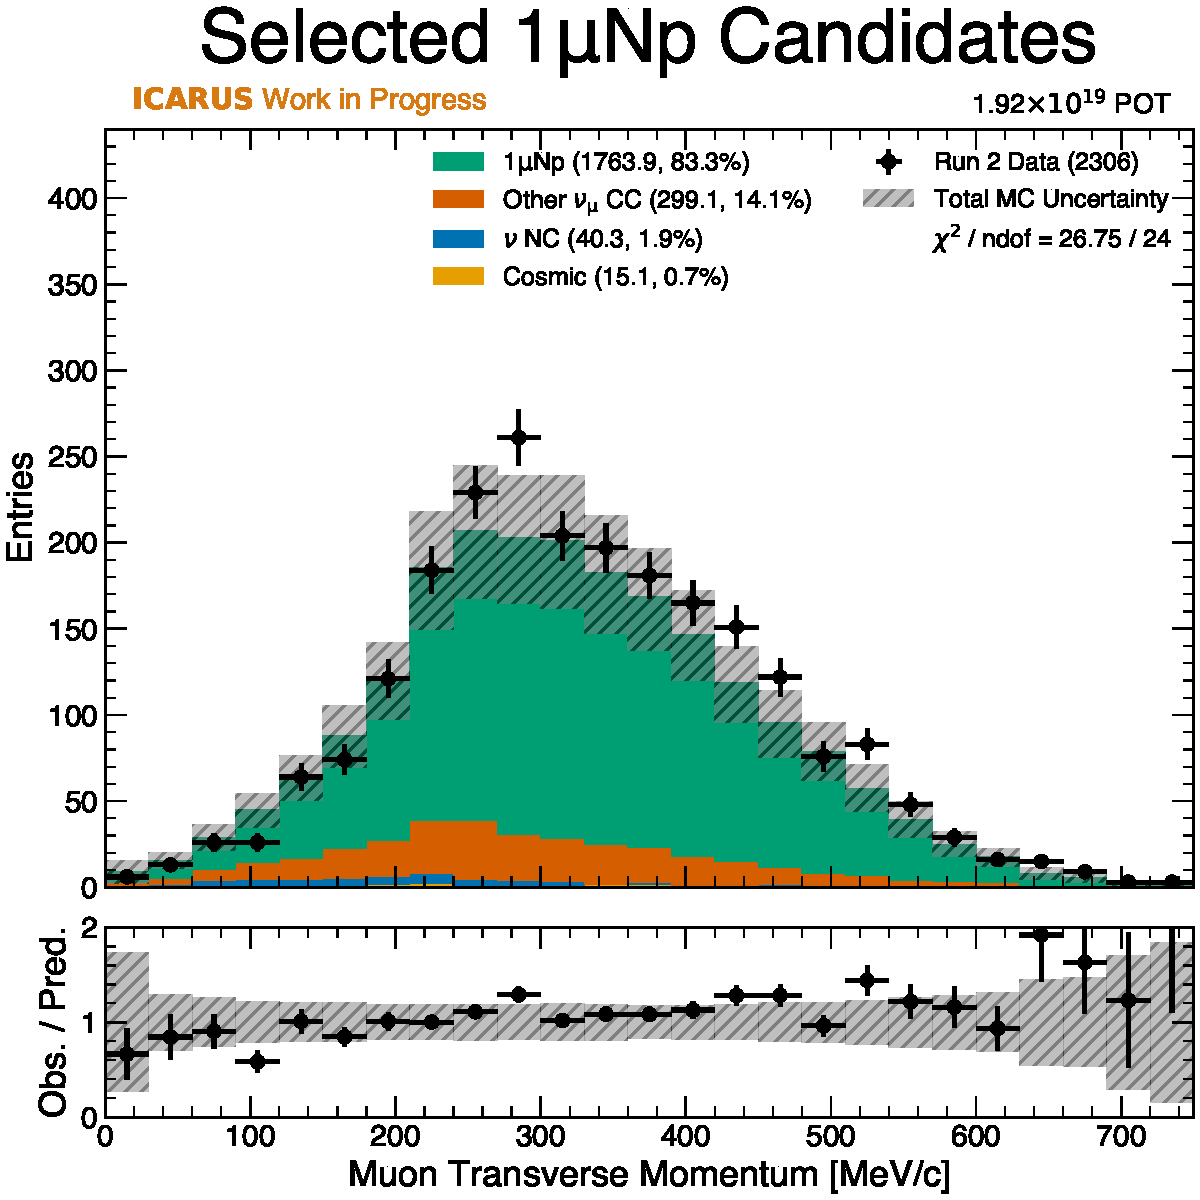
\includegraphics[width=0.41\textwidth]{figures/data_mc_comparisons/datamc_hist1d_1muNp_muon_pt.pdf}
    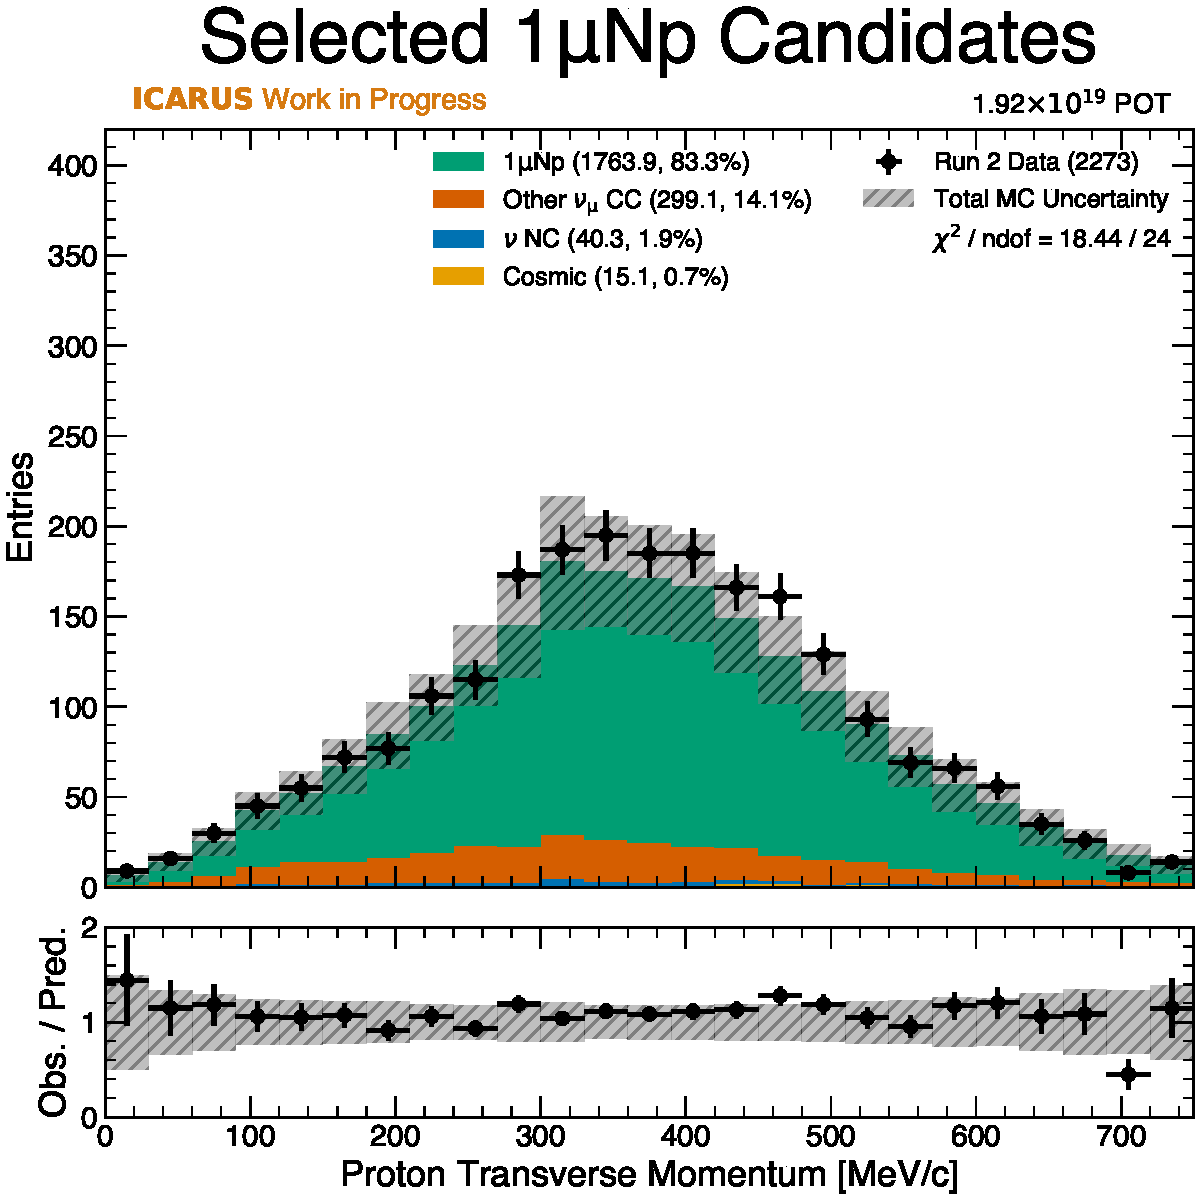
\includegraphics[width=0.41\textwidth]{figures/data_mc_comparisons/datamc_hist1d_1muNp_proton_pt.pdf}
    \\
    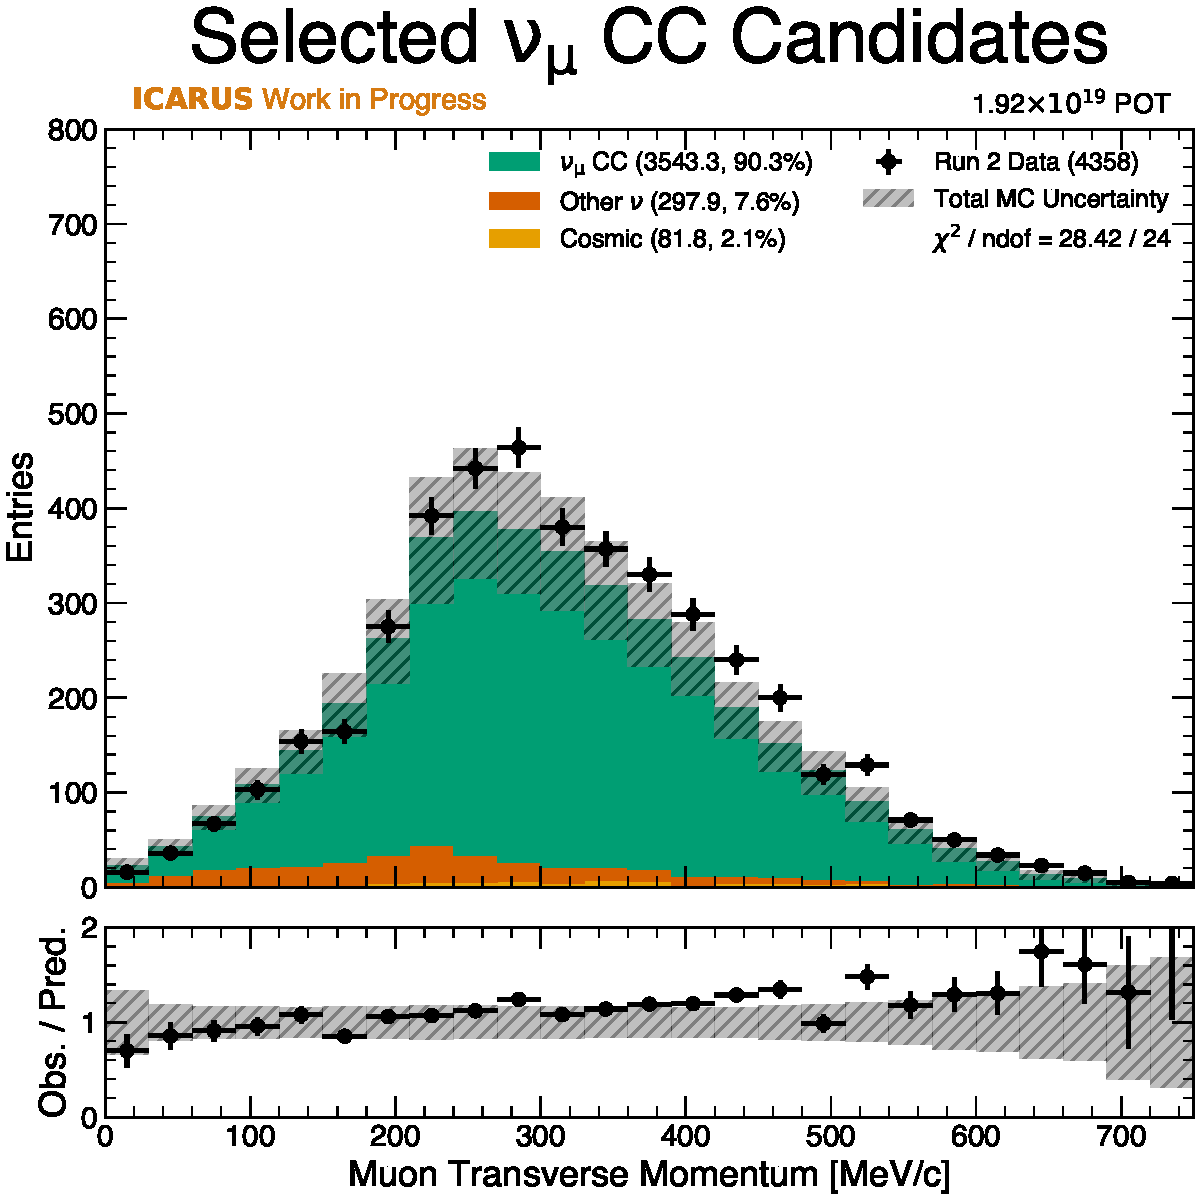
\includegraphics[width=0.41\textwidth]{figures/data_mc_comparisons/datamc_hist1d_1muX_muon_pt.pdf}
    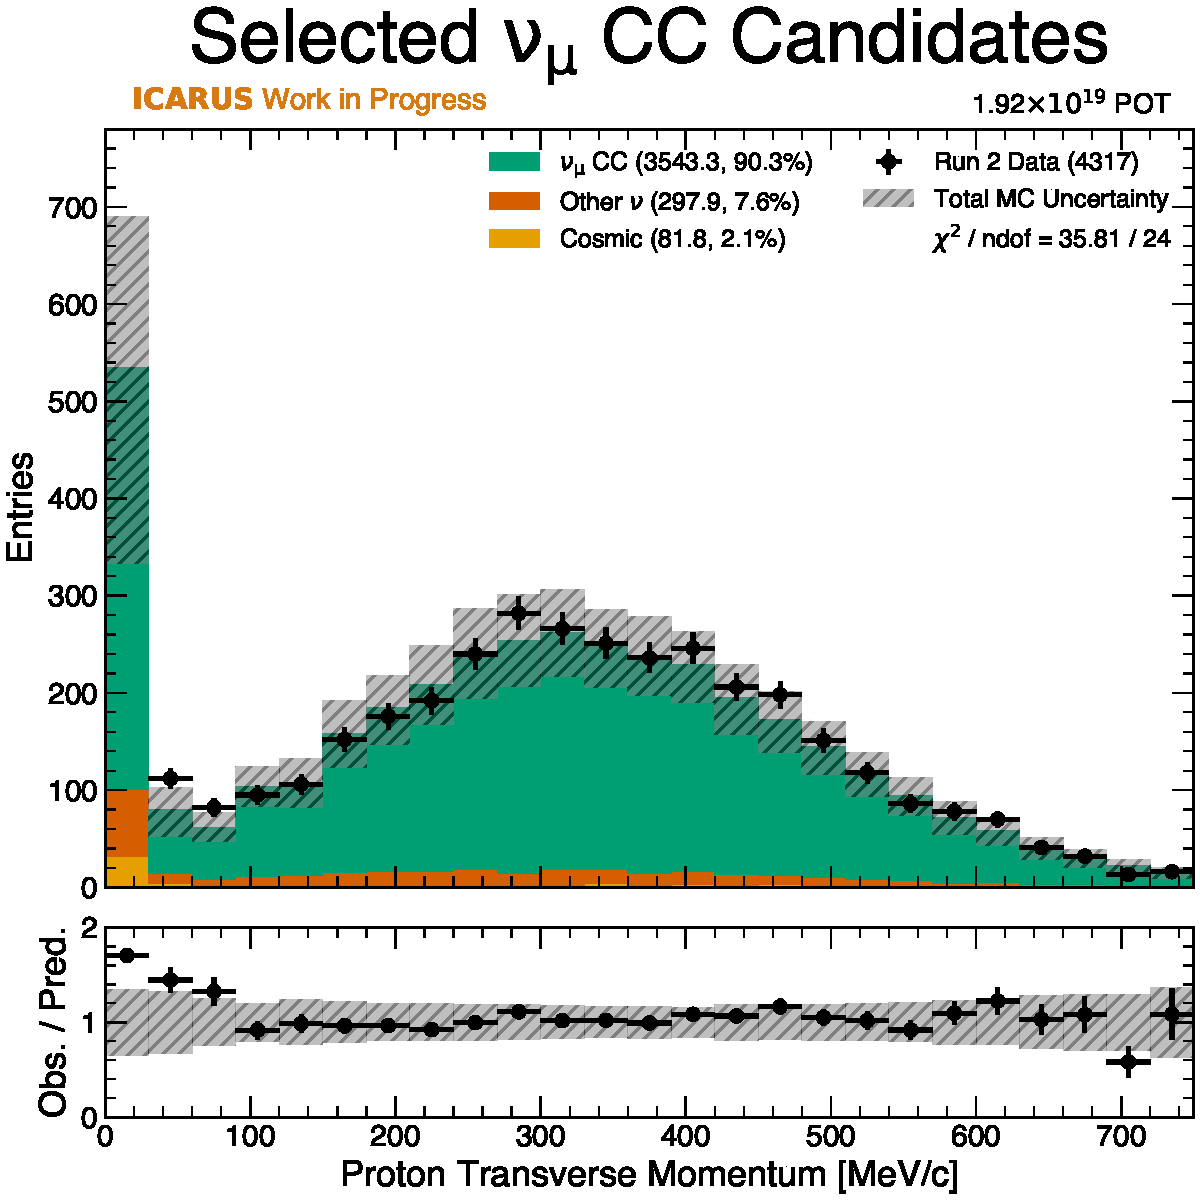
\includegraphics[width=0.41\textwidth]{figures/data_mc_comparisons/datamc_hist1d_1muX_proton_pt.pdf}
    \caption{Comparison of data and simulation for the transverse momentum of the muon (left) and the most energetic proton (right) for each of the three signal channels: from top to bottom $\mathrm{1\mu 1p}$, $\mathrm{1\mu Np}$, and $\nu_\mu$ CC inclusive. The peak in the lowest bin of the proton transverse momentum distribution in the inclusive channel is from interactions that do not have a proton in the final state.}
    \label{fig:datamc_muon_proton_pt}
\end{figure}

\begin{figure}
    \centering
    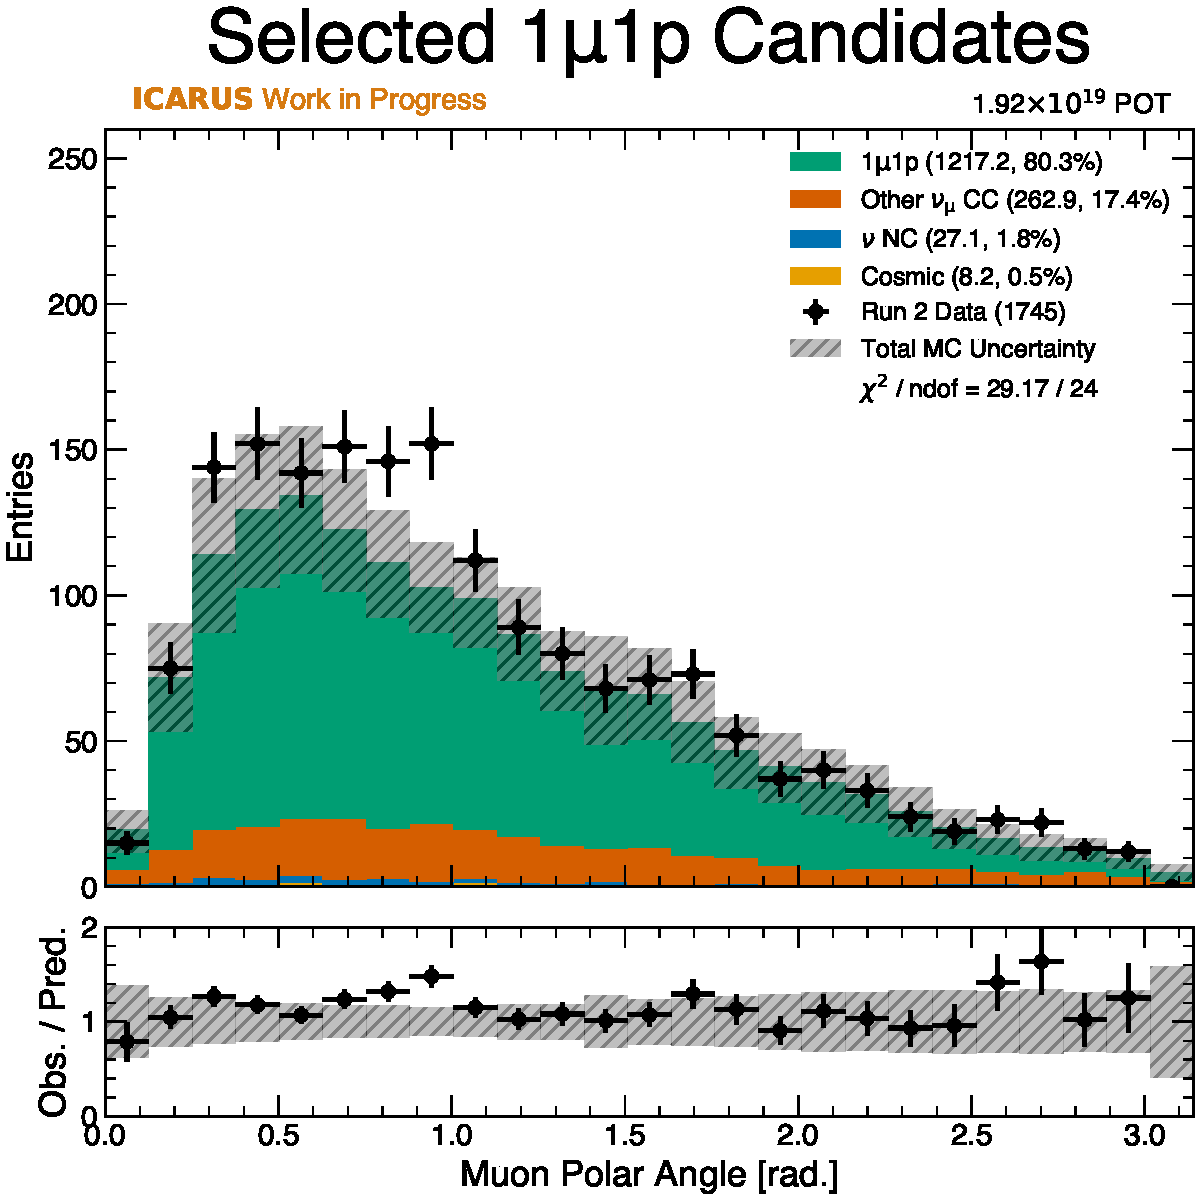
\includegraphics[width=0.42\textwidth]{figures/data_mc_comparisons/datamc_hist1d_1mu1p_muon_polar_angle.pdf}
    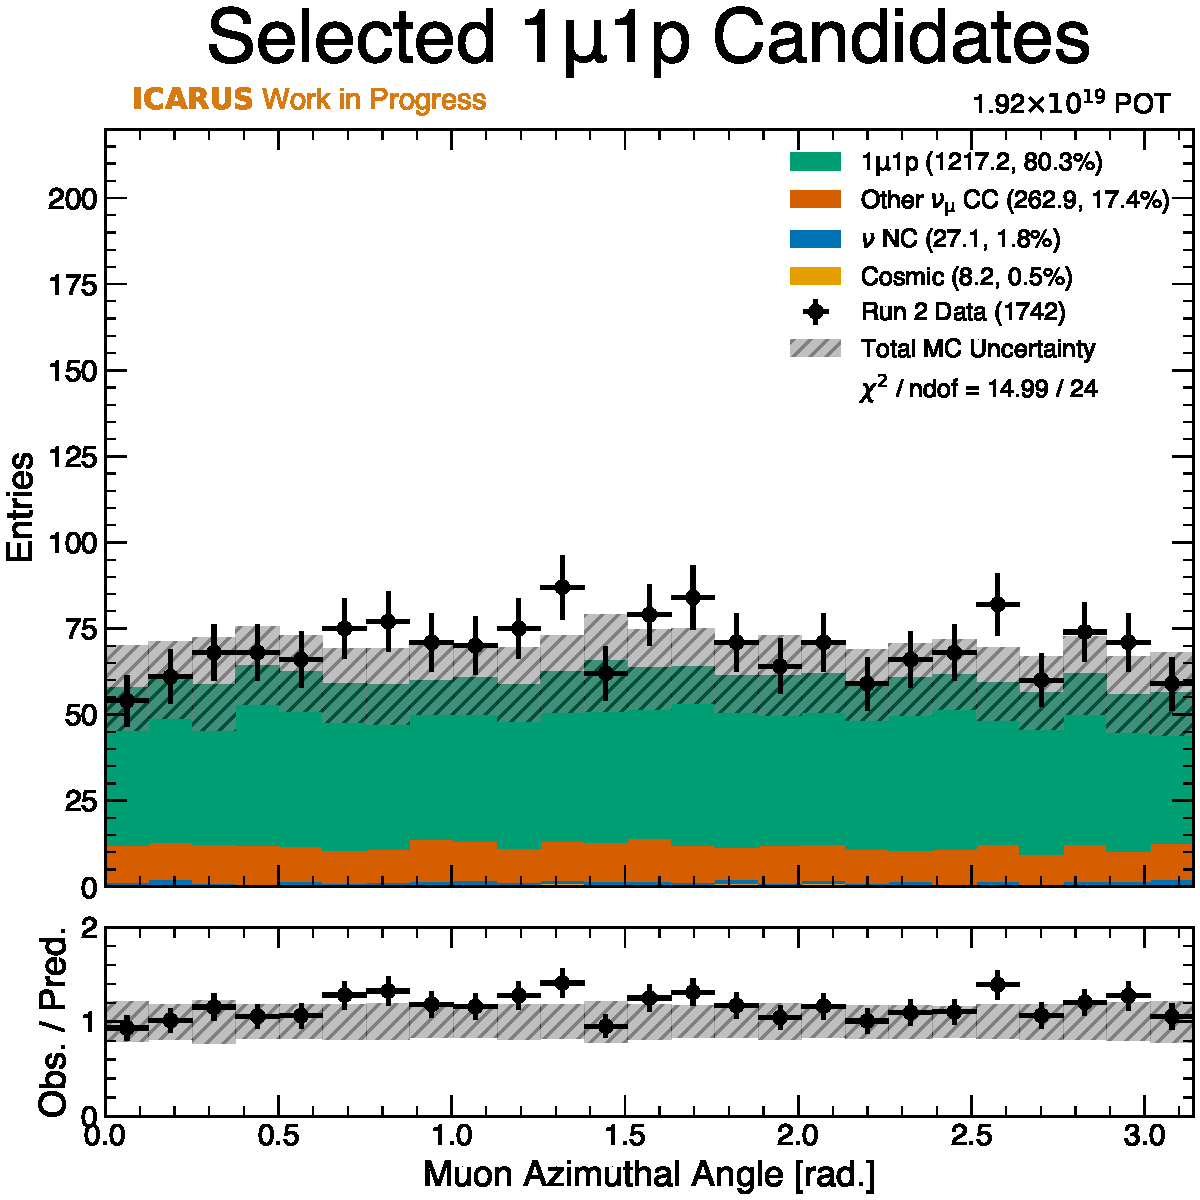
\includegraphics[width=0.42\textwidth]{figures/data_mc_comparisons/datamc_hist1d_1mu1p_muon_azimuthal_angle.pdf}
    \\
    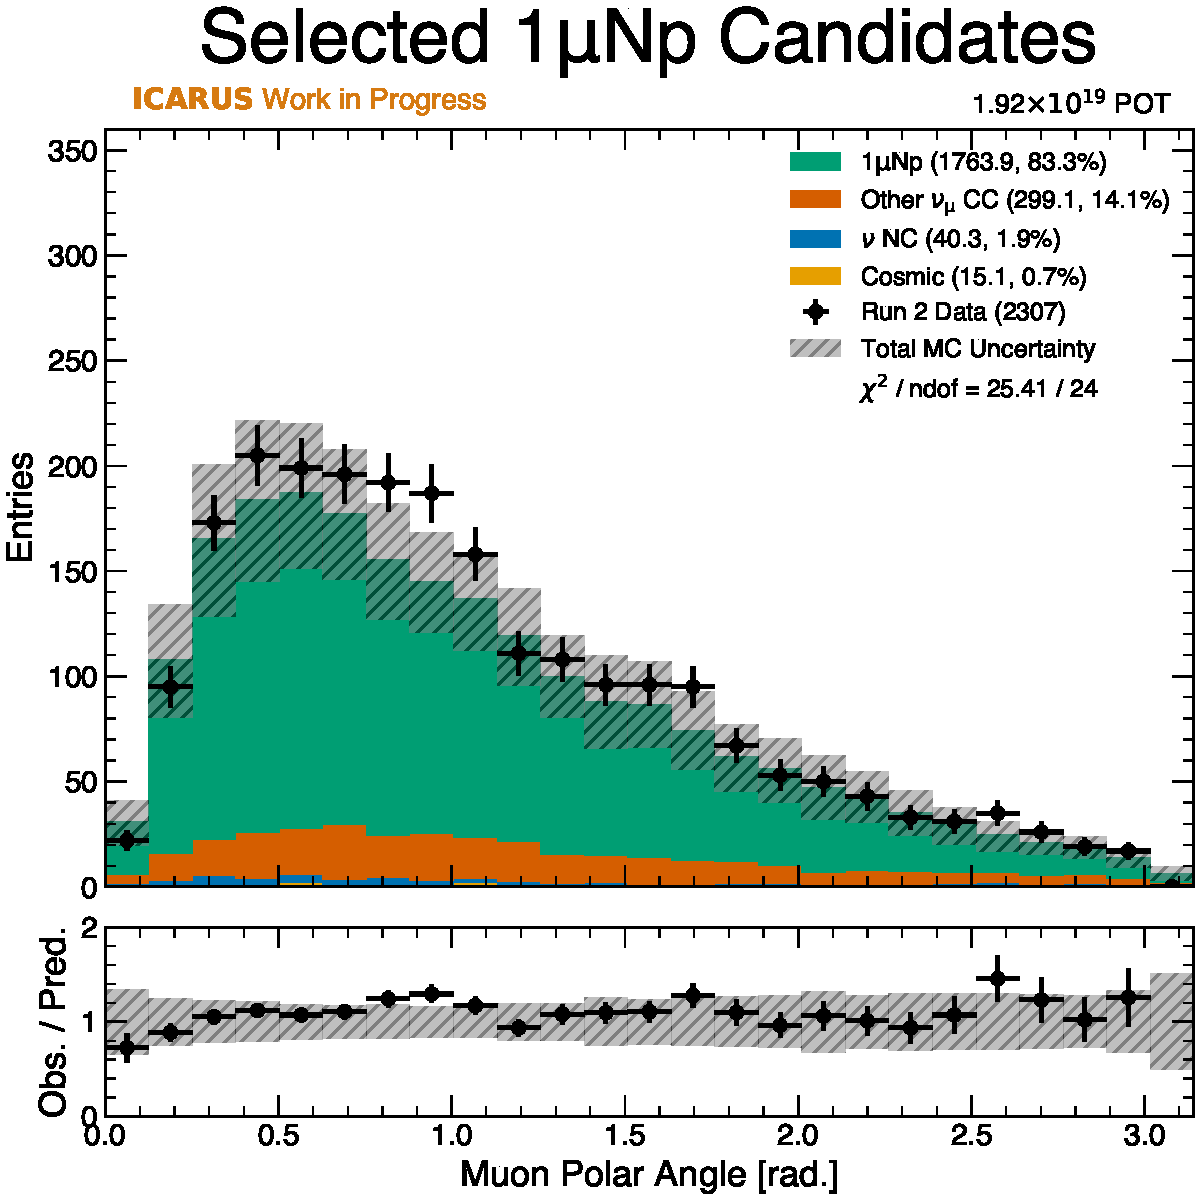
\includegraphics[width=0.42\textwidth]{figures/data_mc_comparisons/datamc_hist1d_1muNp_muon_polar_angle.pdf}
    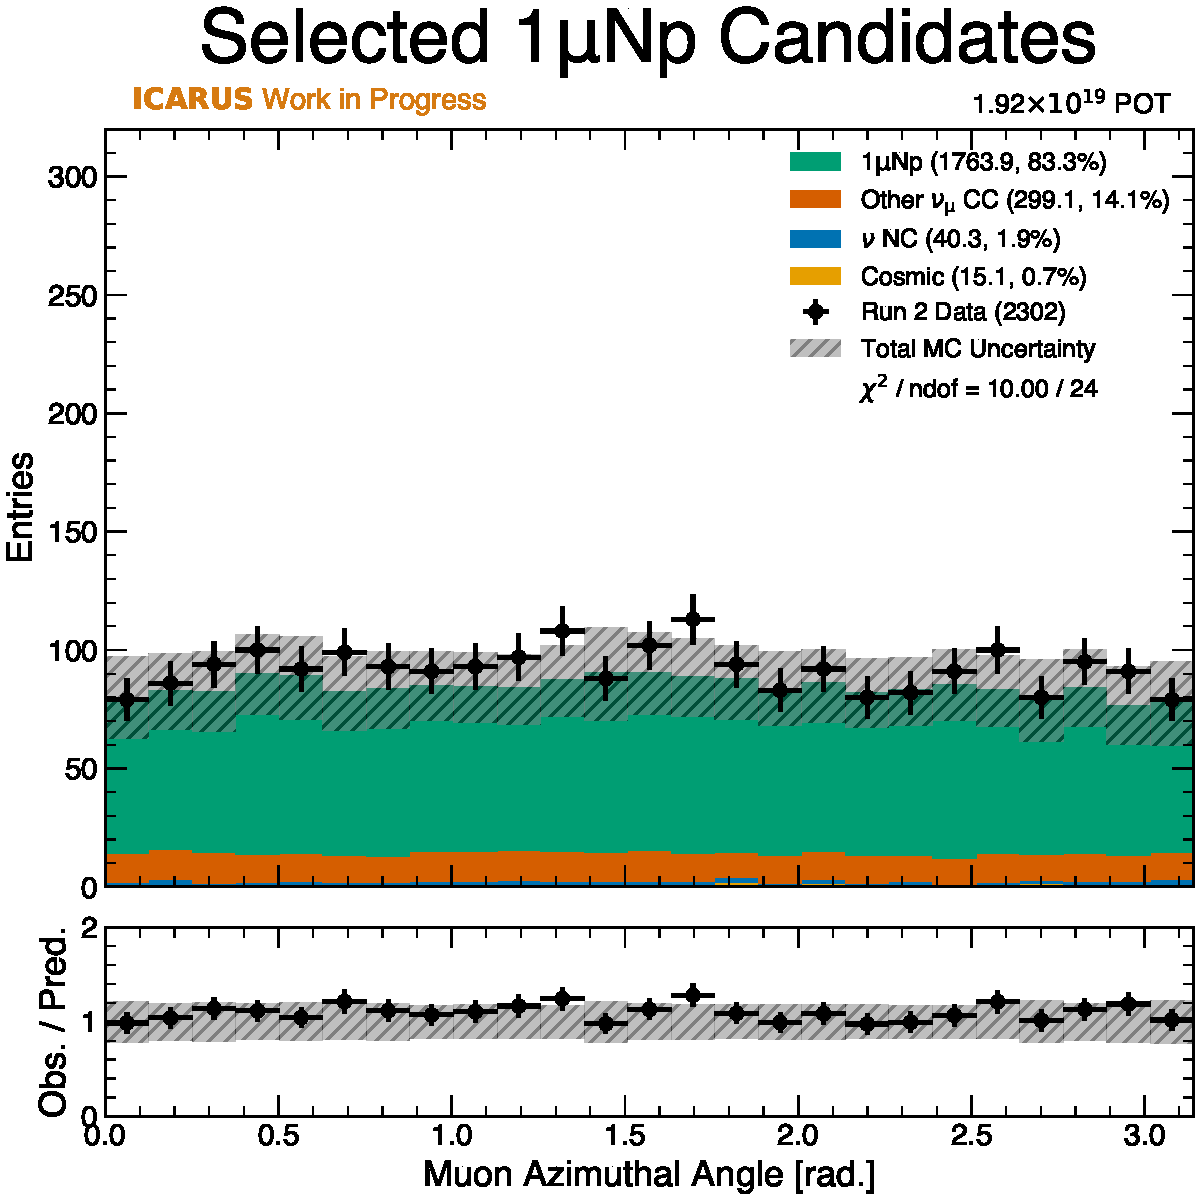
\includegraphics[width=0.42\textwidth]{figures/data_mc_comparisons/datamc_hist1d_1muNp_muon_azimuthal_angle.pdf}
    \\
    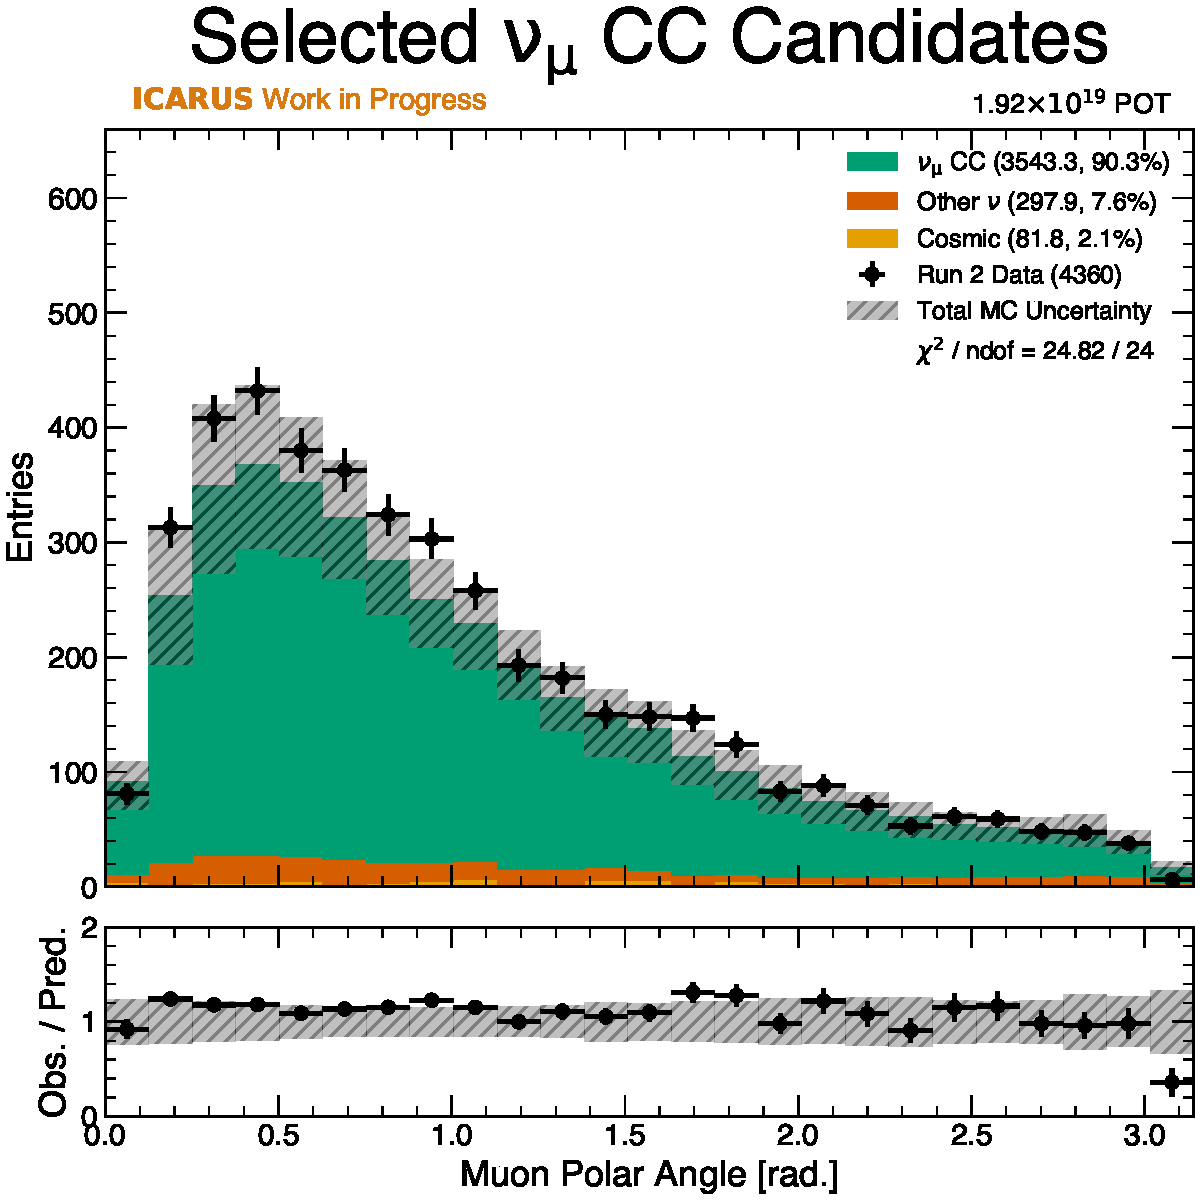
\includegraphics[width=0.42\textwidth]{figures/data_mc_comparisons/datamc_hist1d_1muX_muon_polar_angle.pdf}
    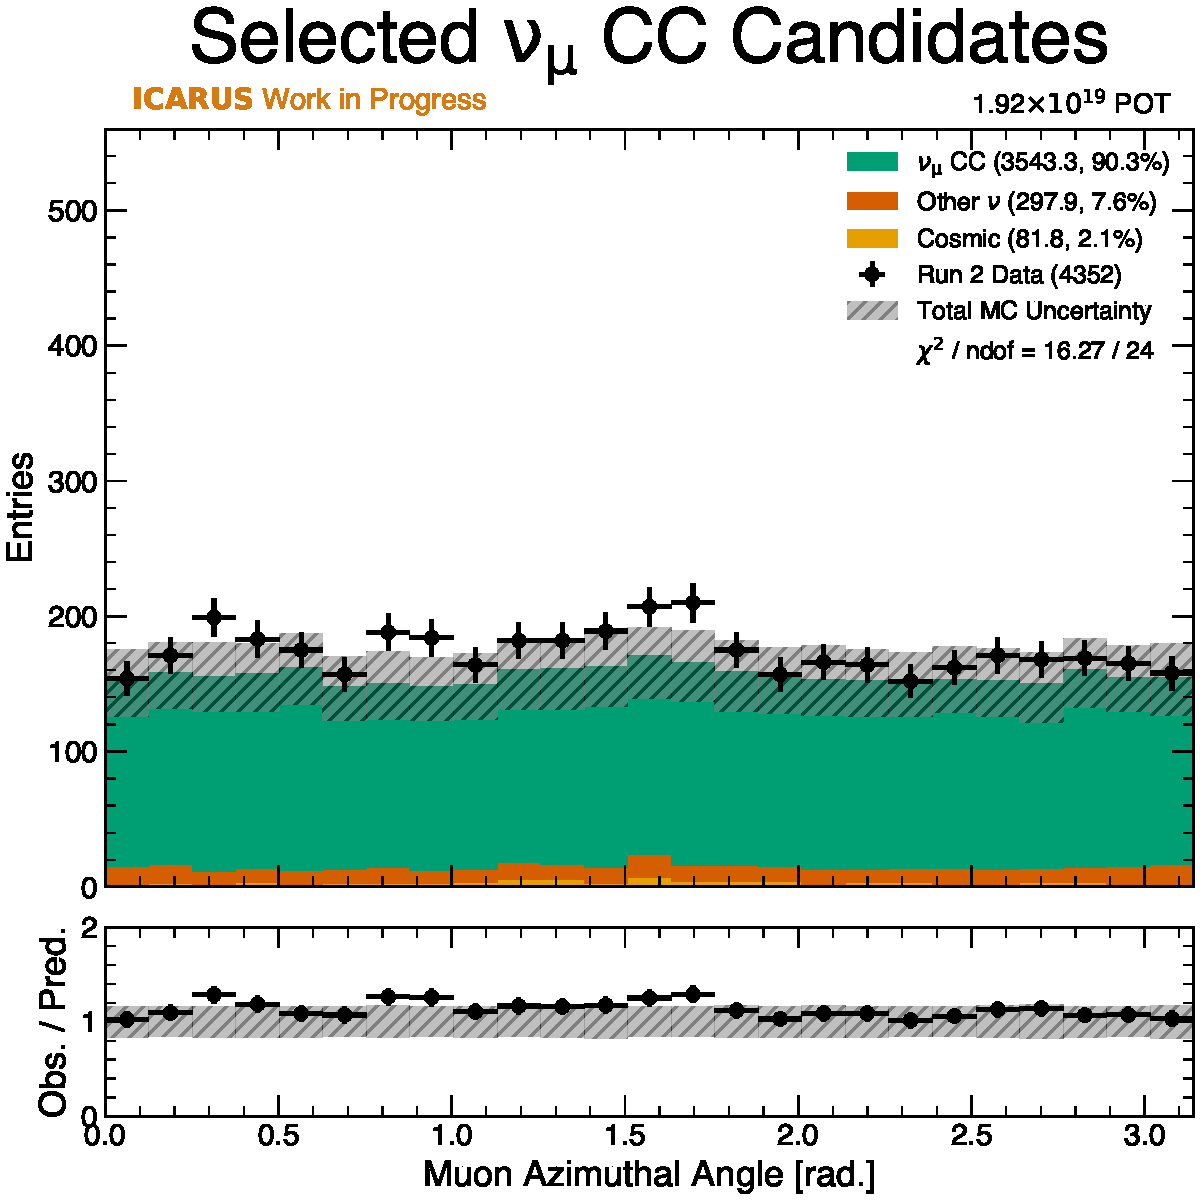
\includegraphics[width=0.42\textwidth]{figures/data_mc_comparisons/datamc_hist1d_1muX_muon_azimuthal_angle.pdf}
    \caption{Comparison of data and simulation for the polar angle (left) and azimuthal angle (right) of the muon for each of the three signal channels: from top to bottom $\mathrm{1\mu 1p}$, $\mathrm{1\mu Np}$, and $\nu_\mu$ CC inclusive.}
    \label{fig:datamc_muon_angles}
\end{figure}

Comparisons of data and simulation are presented in Figures \ref{fig:datamc_muon_proton_ke} through \ref{fig:datamc_muon_angles} for the interaction kinematic variables defined in Section \ref{sec:interaction_kinematic_variables}. Generally, an excess of events is observed in the data compared to simulation, but the difference is near the expected uncertainty. The muon and proton energy distributions seem to have shifts in the distribution that are opposite: the muon energy distribution is shifted to higher energies in data compared to simulation, while the proton energy distribution is shifted to lower energies. The total visible energy distribution shows a generally higher amount of events in data compared to simulation, but the shape of the distribution matches well.

There are no significant deviations in the muon and proton transverse momentum distributions, the muon polar and azimuthal angle distributions, or the muon-proton opening angle distributions. Many reconstruction inefficiencies, such as signal removal from coherent noise filtering, could potentially impact these distributions, so it is especially important that we see good agreement in these variables. 

\subsubsection{Comparisons for Kinematic Imbalance Variables}
\label{sec:datamc_kinematic_imbalance_variables}

\begin{figure}
    \centering
    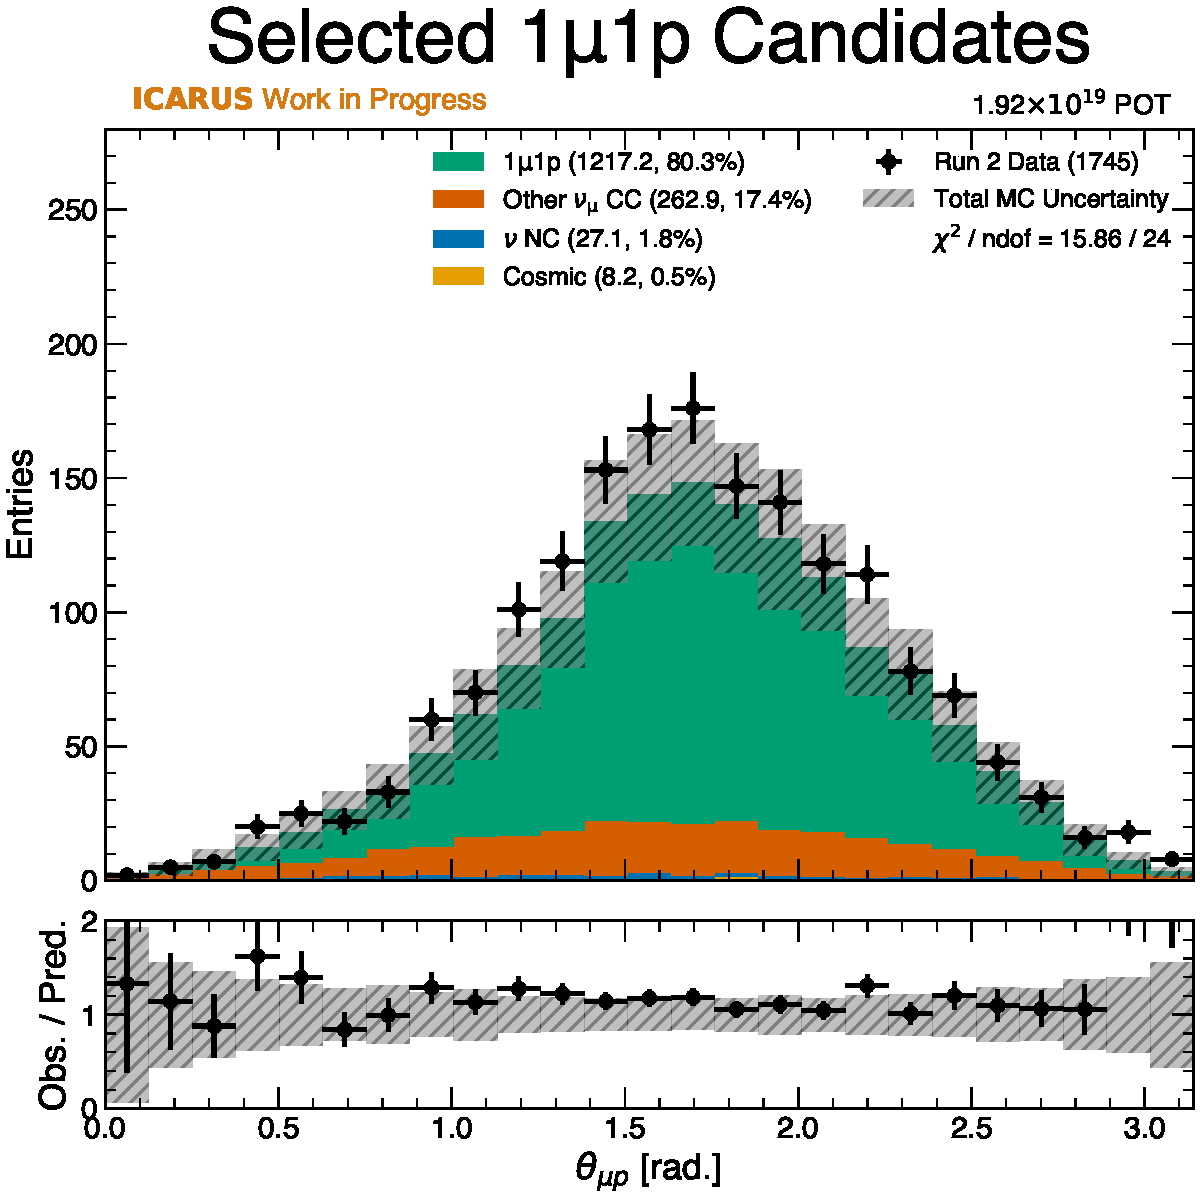
\includegraphics[width=0.41\textwidth]{figures/data_mc_comparisons/datamc_hist1d_1mu1p_opening_angle.pdf}\\
    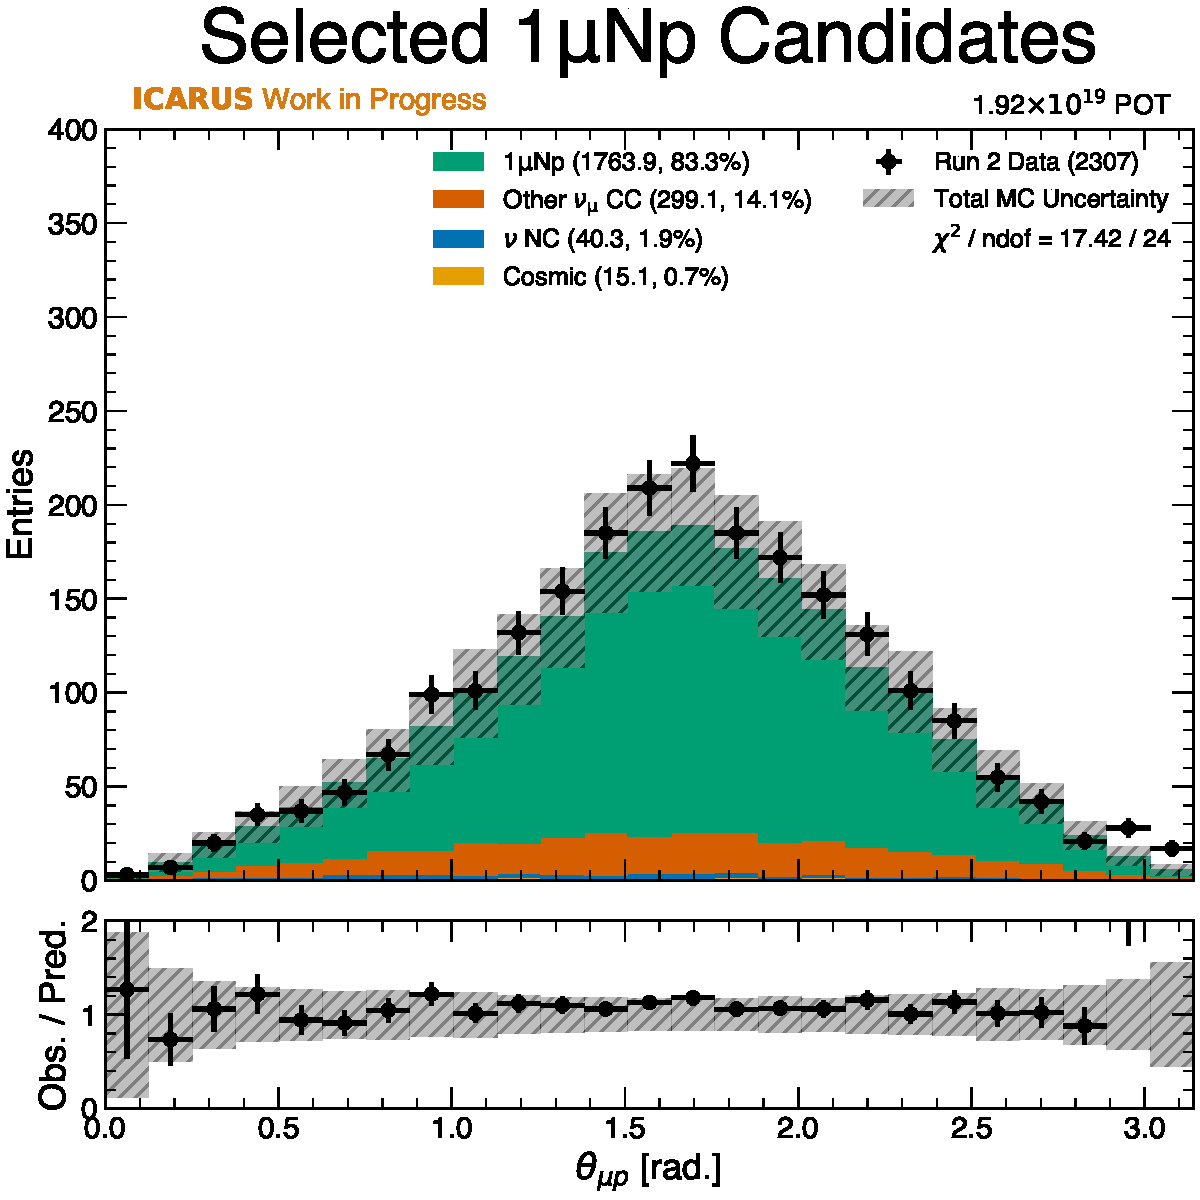
\includegraphics[width=0.41\textwidth]{figures/data_mc_comparisons/datamc_hist1d_1muNp_opening_angle.pdf}\\
    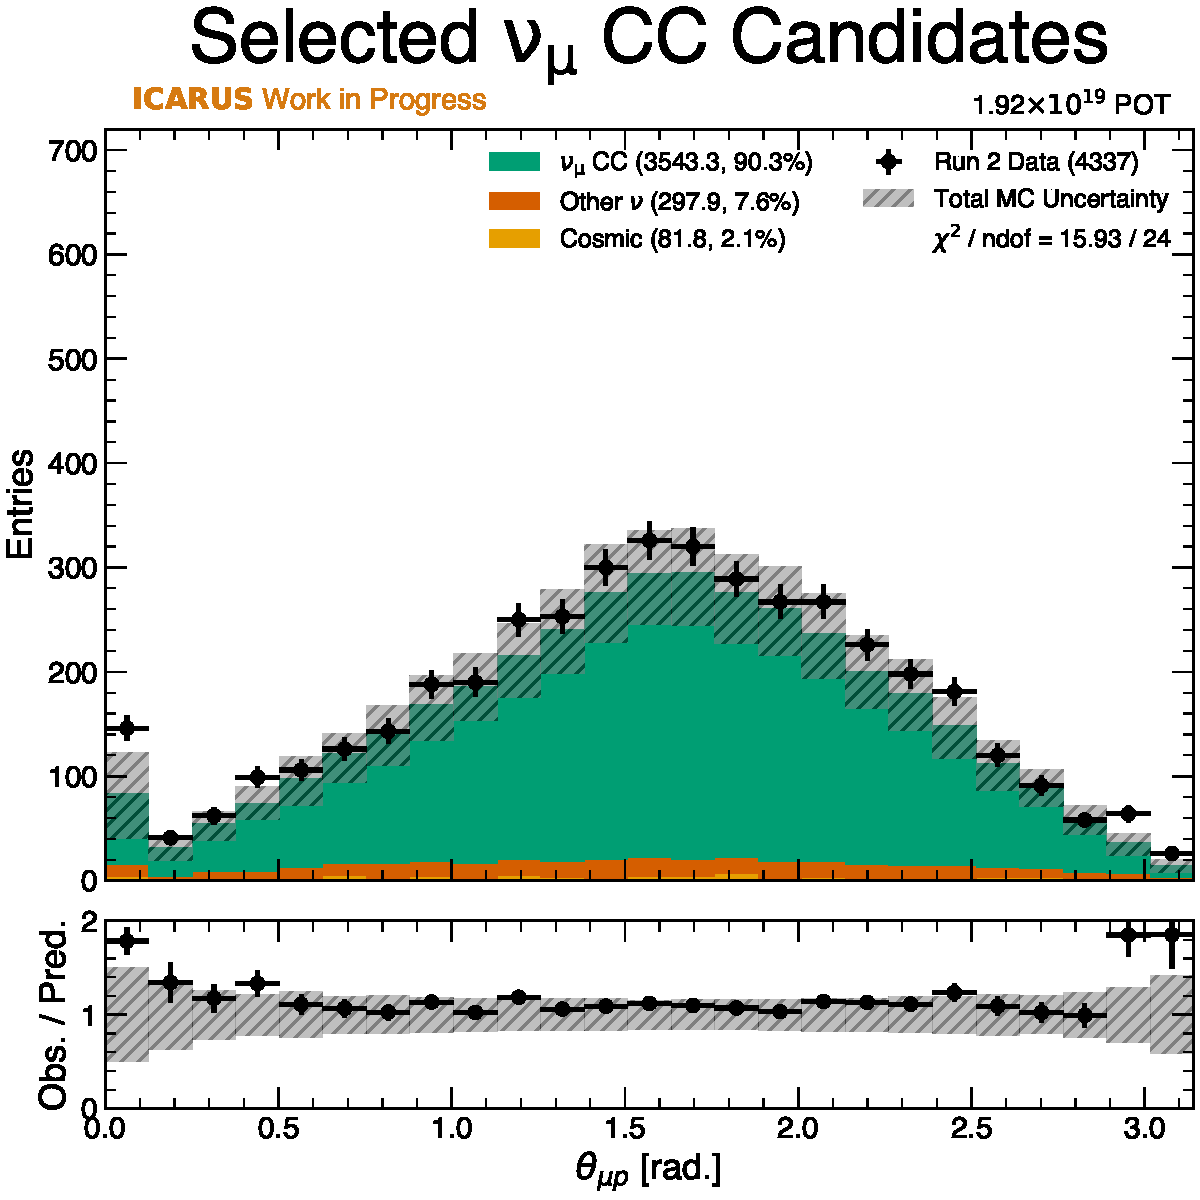
\includegraphics[width=0.41\textwidth]{figures/data_mc_comparisons/datamc_hist1d_1muX_opening_angle.pdf}\\
    \caption{Comparison of data and simulation for the the muon-proton opening angle for each of the three signal channels: from top to bottom $\mathrm{1\mu 1p}$, $\mathrm{1\mu Np}$, and $\nu_\mu$ CC inclusive. The peak in the lowest bin of the proton transverse momentum distribution in the inclusive channel is from interactions that do not have a proton in the final state.}
    \label{fig:datamc_opening_angle}
\end{figure}

\begin{figure}
    \centering
    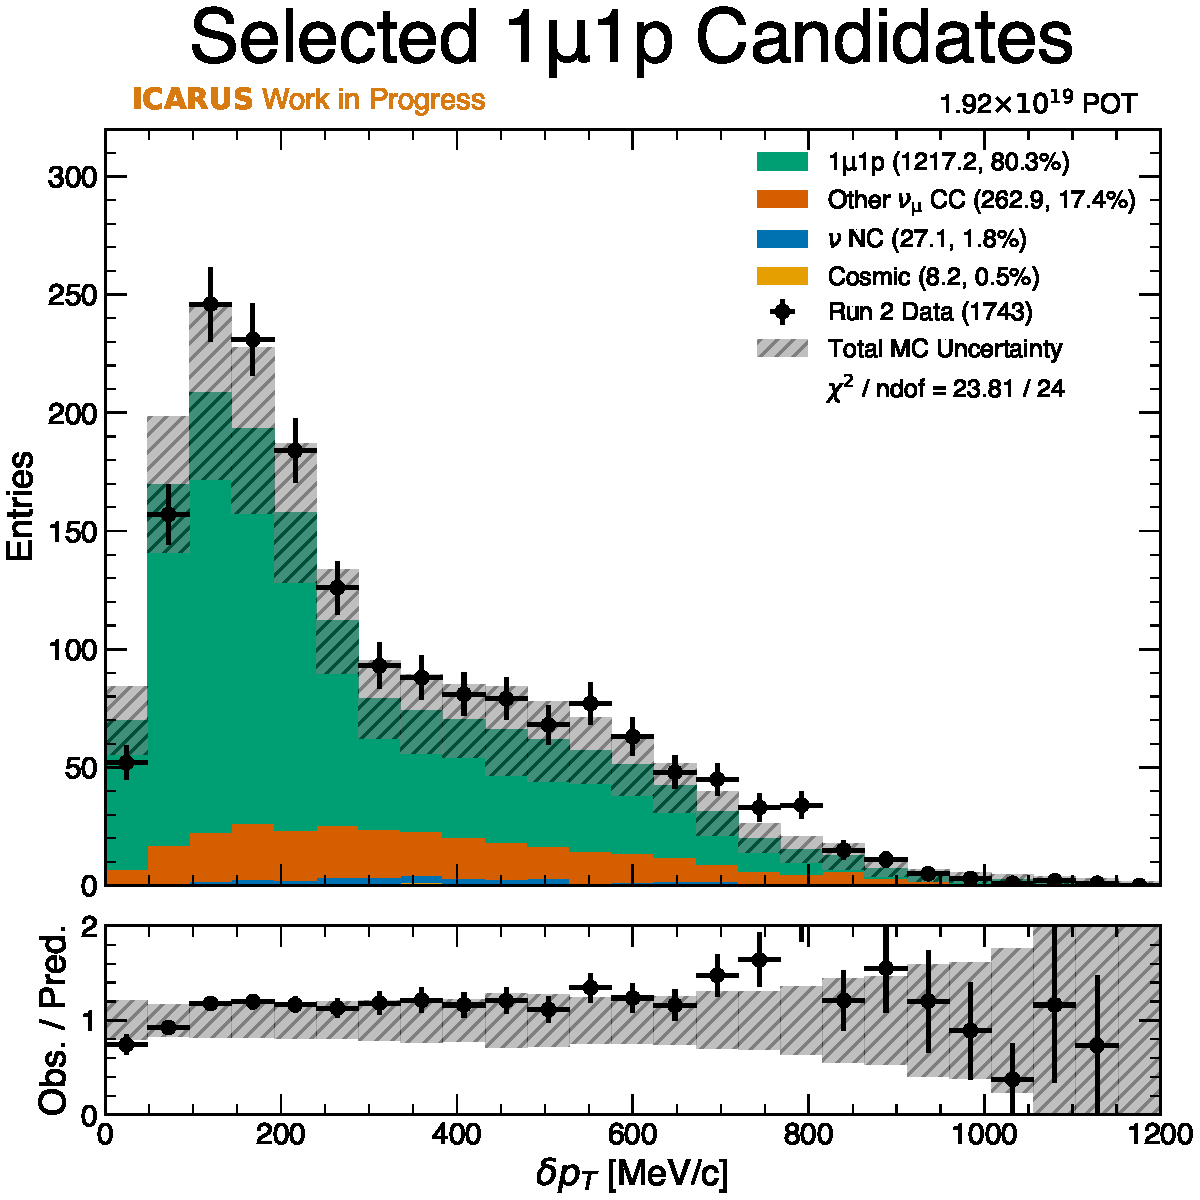
\includegraphics[width=0.42\textwidth]{figures/data_mc_comparisons/datamc_hist1d_1mu1p_delta_pT.pdf}\\
    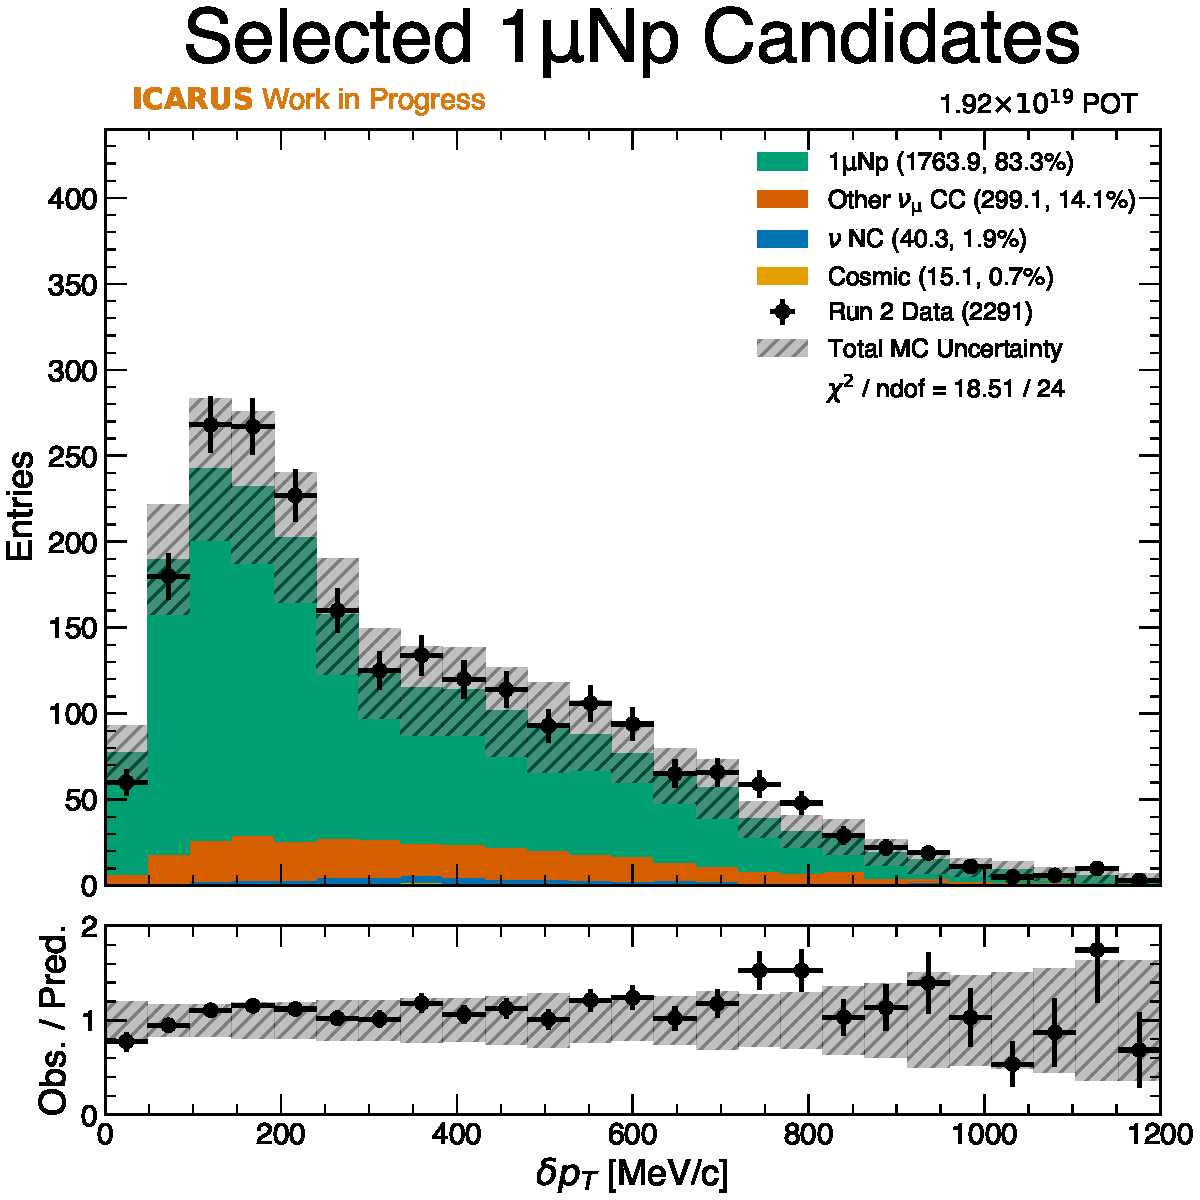
\includegraphics[width=0.42\textwidth]{figures/data_mc_comparisons/datamc_hist1d_1muNp_delta_pT.pdf}\\
    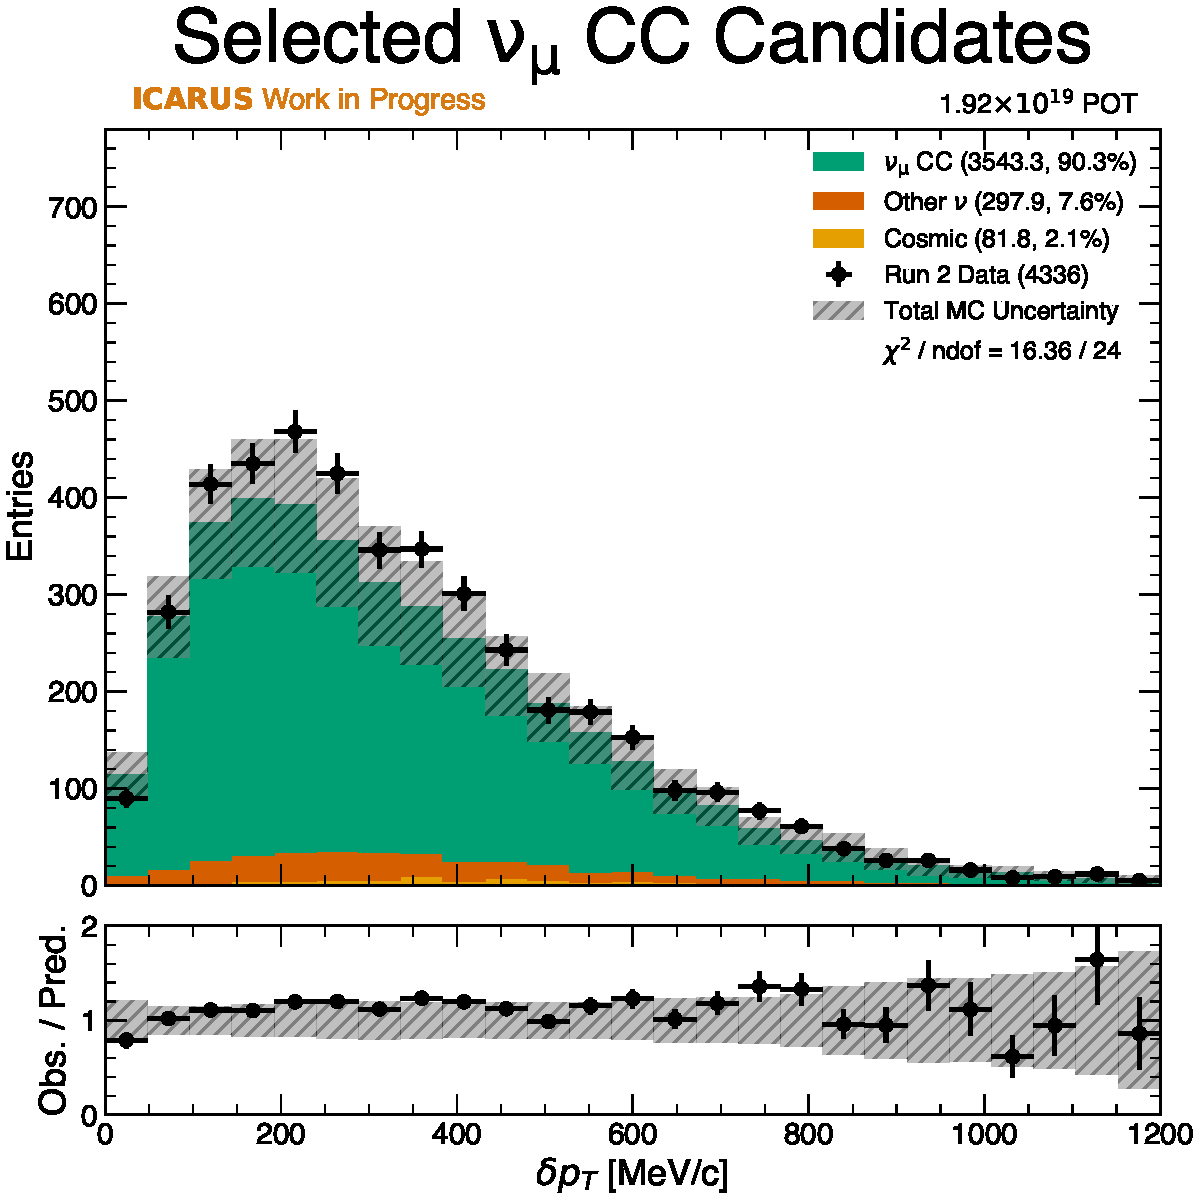
\includegraphics[width=0.42\textwidth]{figures/data_mc_comparisons/datamc_hist1d_1muX_delta_pT.pdf}\\
    \caption{Comparison of data and simulation for the transverse momentum of the interaction for each of the three signal channels: from top to bottom $\mathrm{1\mu 1p}$, $\mathrm{1\mu Np}$, and $\nu_\mu$ CC inclusive.}
    \label{fig:datamc_delta_pT}
\end{figure}

\begin{figure}
    \centering
    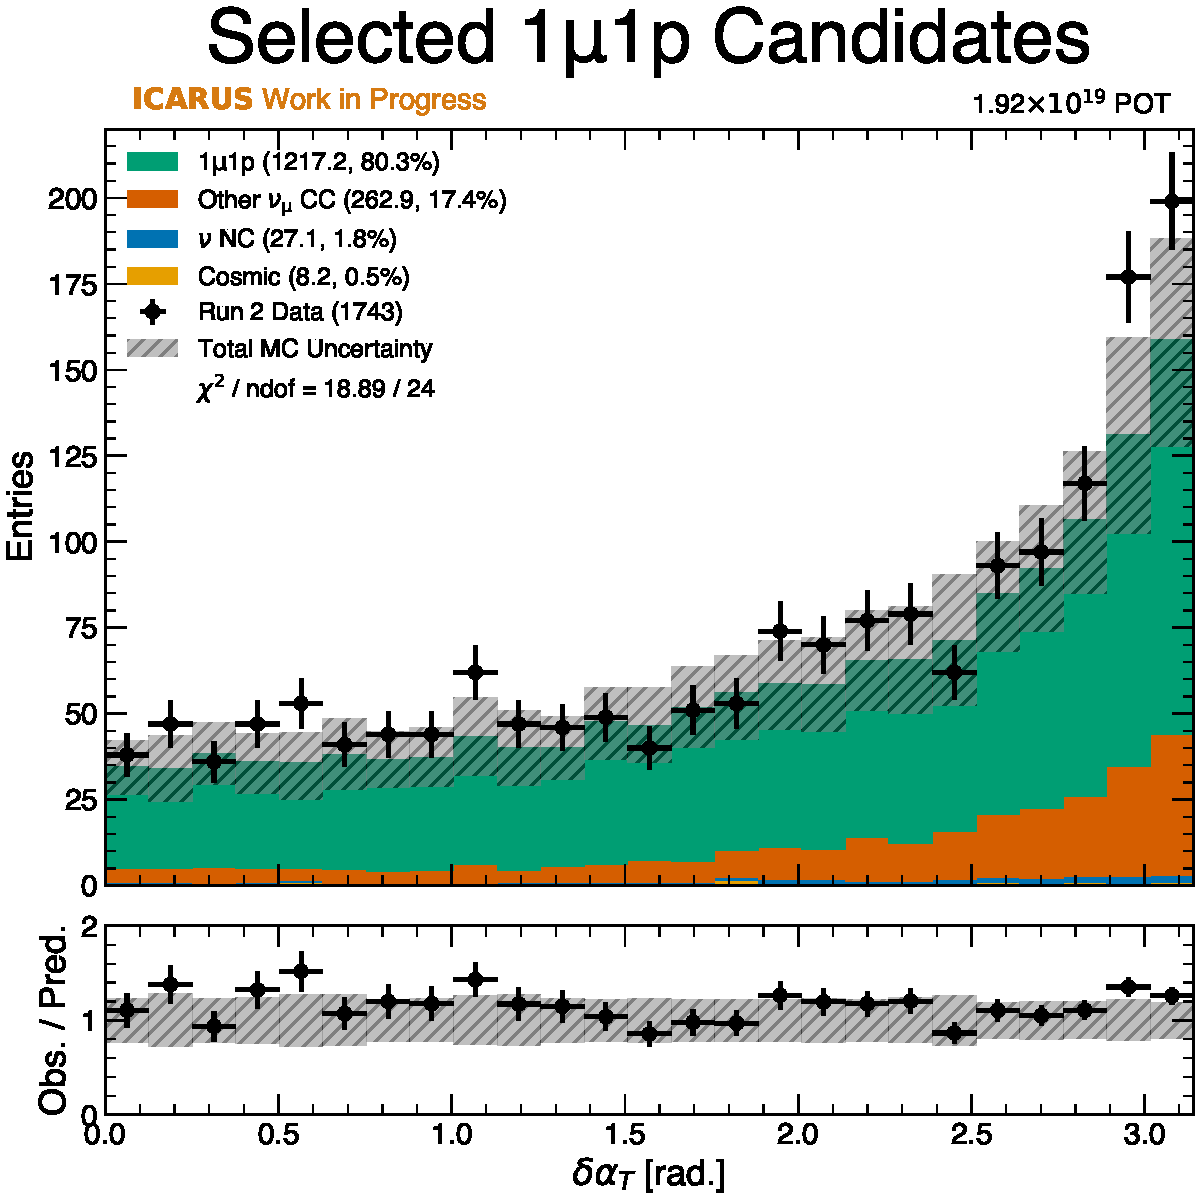
\includegraphics[width=0.42\textwidth]{figures/data_mc_comparisons/datamc_hist1d_1mu1p_delta_alphaT.pdf}
    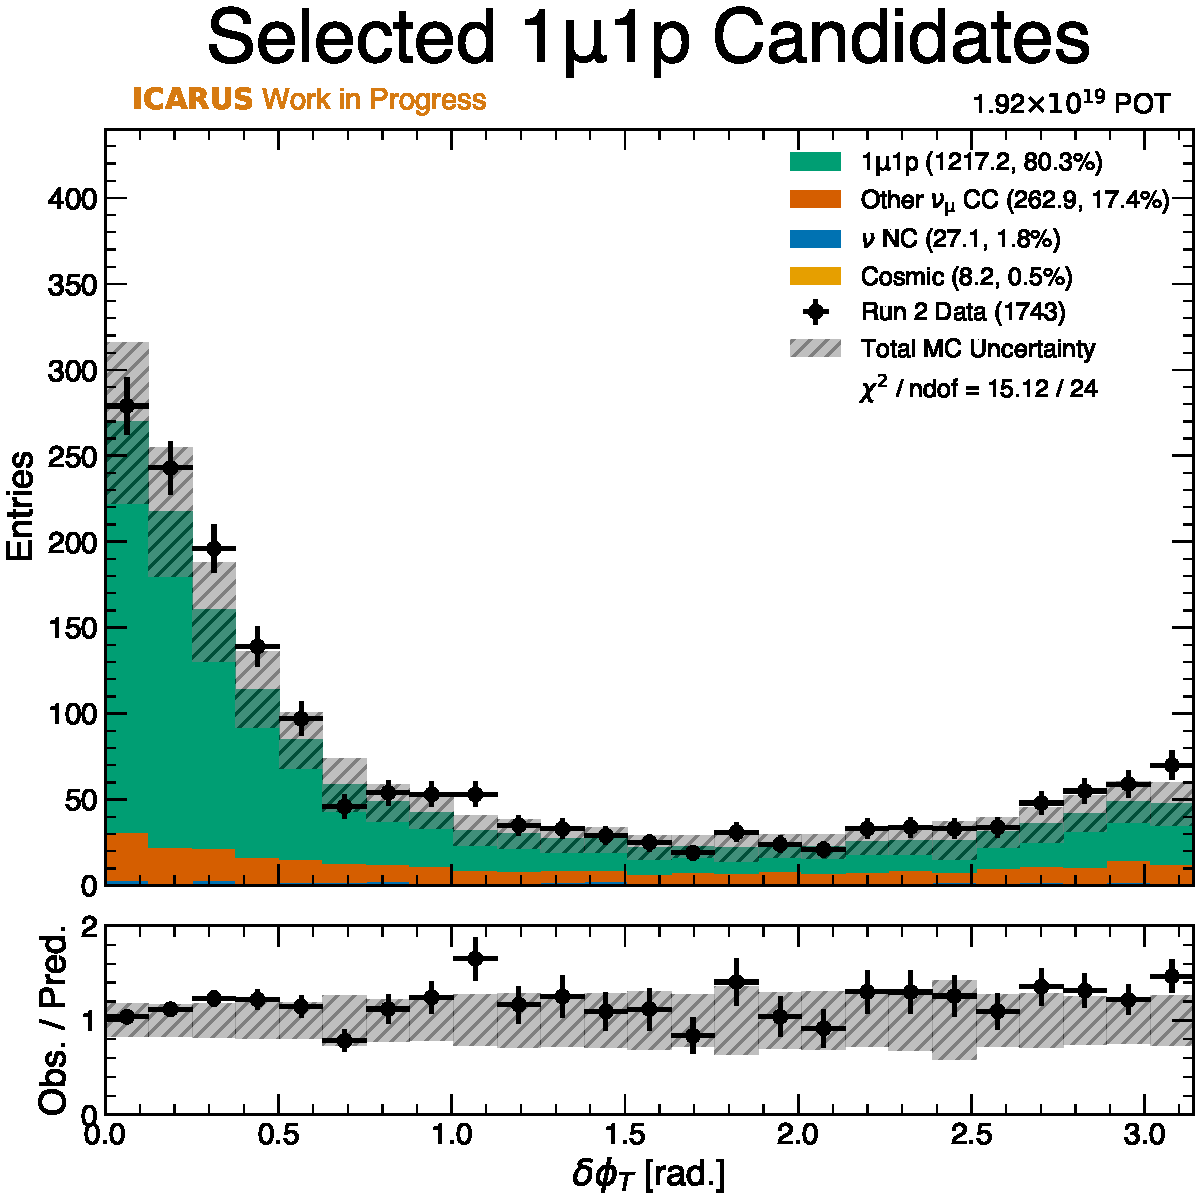
\includegraphics[width=0.42\textwidth]{figures/data_mc_comparisons/datamc_hist1d_1mu1p_delta_phiT.pdf}
    \\
    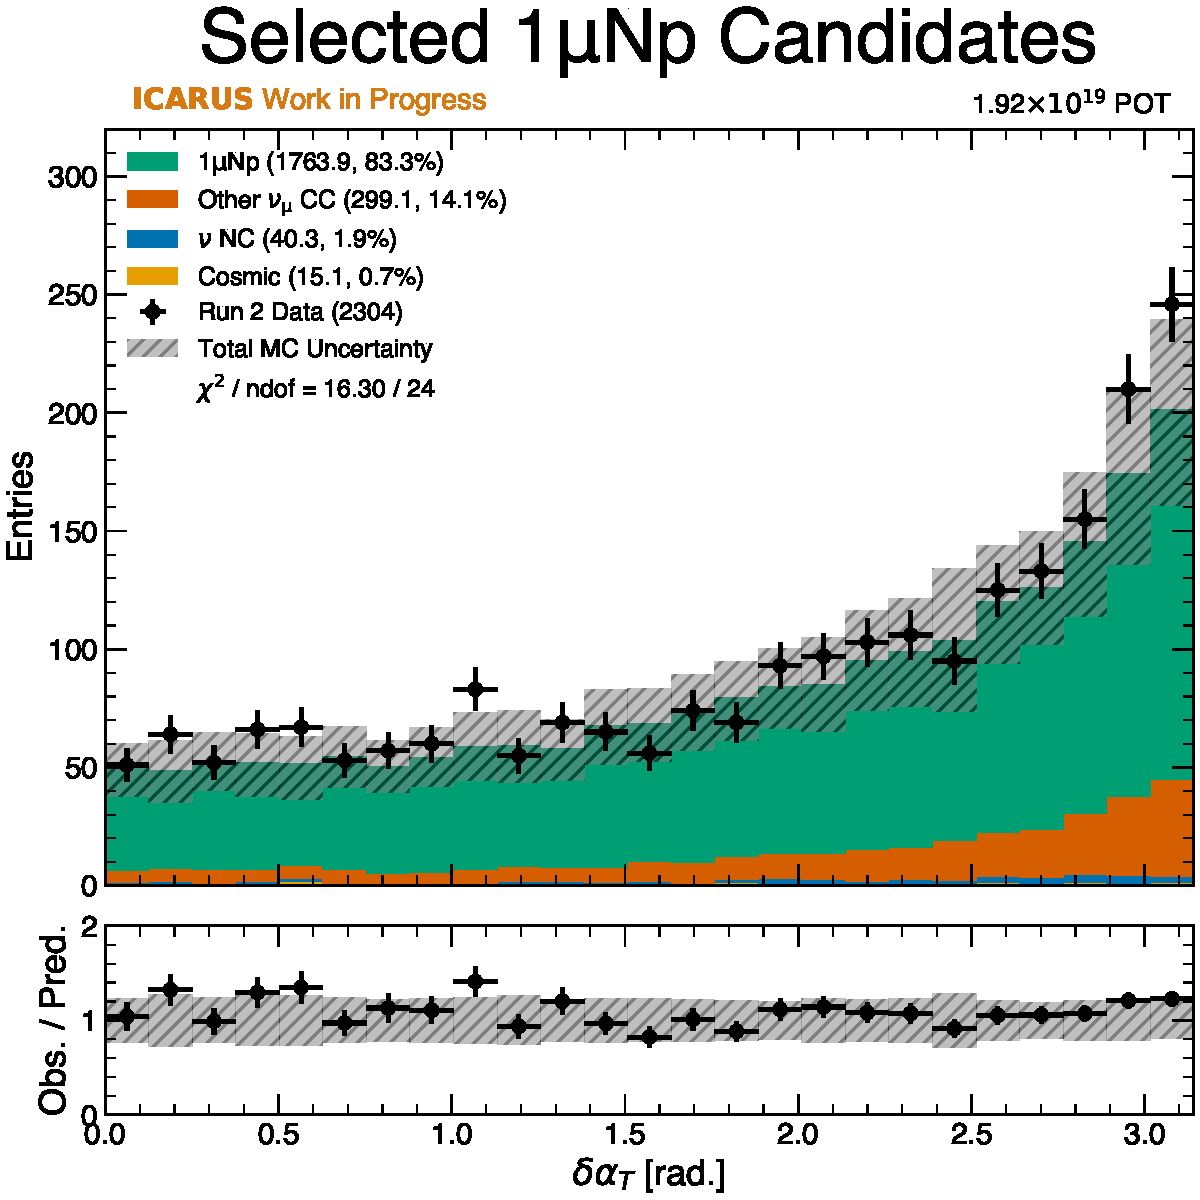
\includegraphics[width=0.42\textwidth]{figures/data_mc_comparisons/datamc_hist1d_1muNp_delta_alphaT.pdf}
    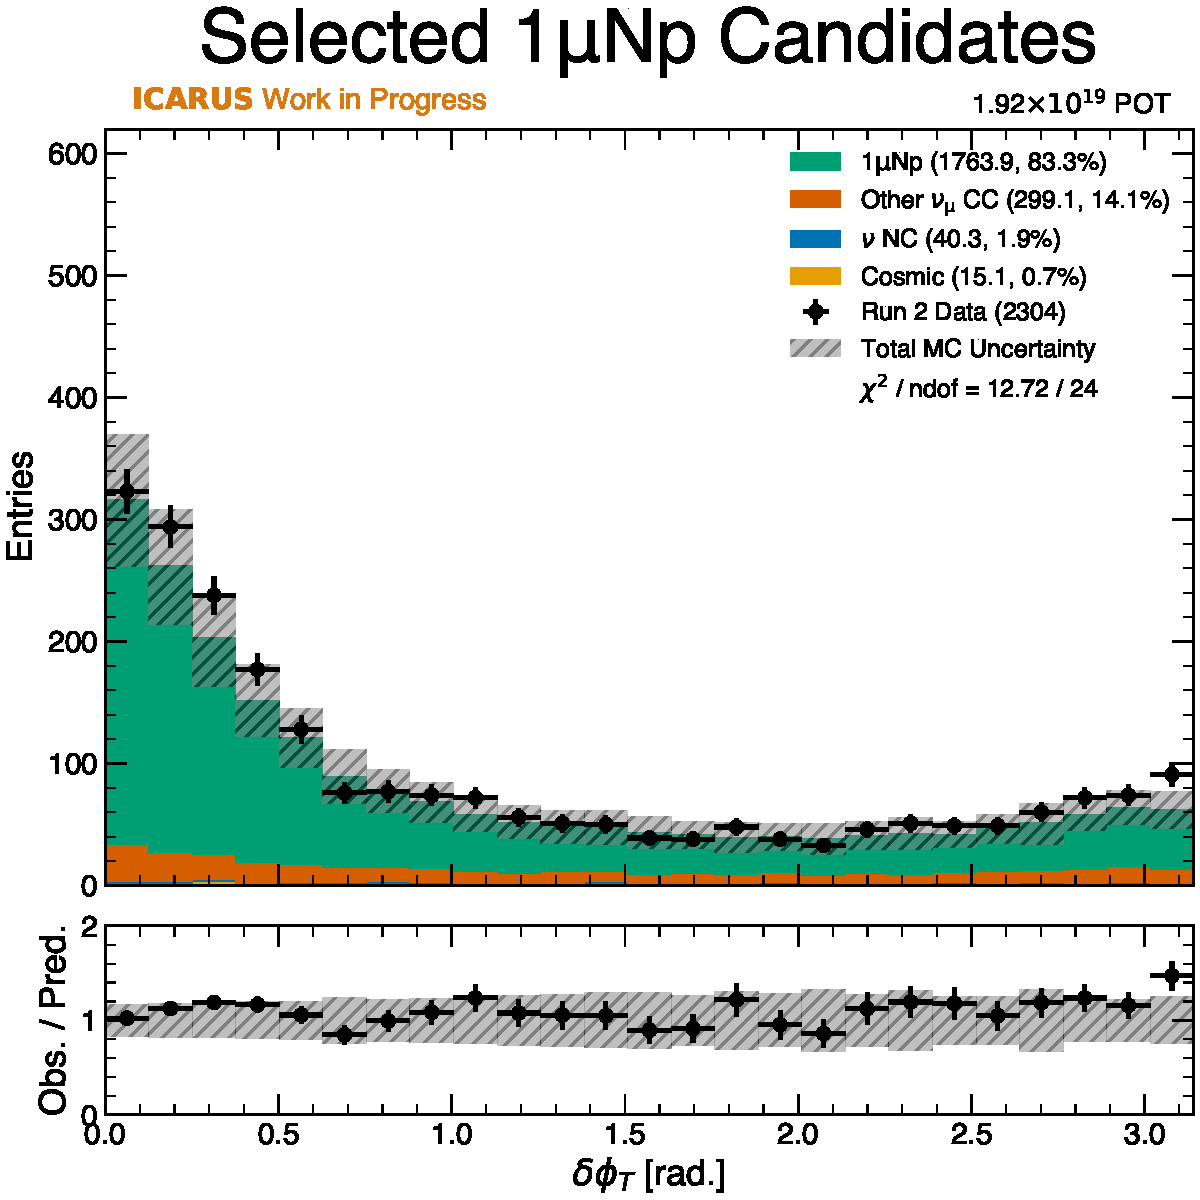
\includegraphics[width=0.42\textwidth]{figures/data_mc_comparisons/datamc_hist1d_1muNp_delta_phiT.pdf}
    \\
    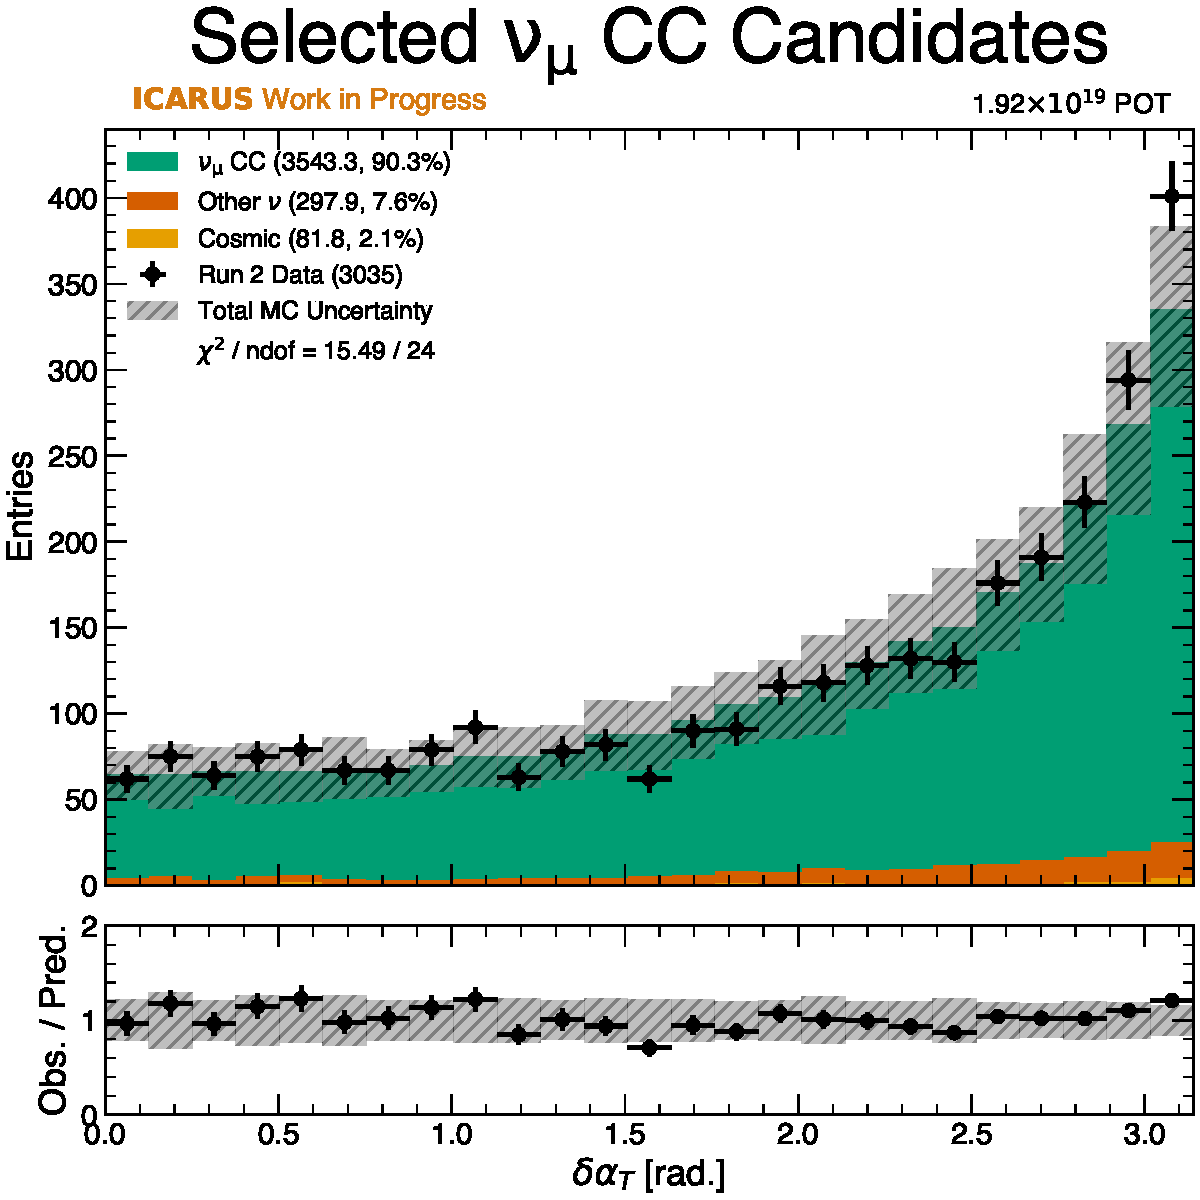
\includegraphics[width=0.42\textwidth]{figures/data_mc_comparisons/datamc_hist1d_1muX_delta_alphaT.pdf}
    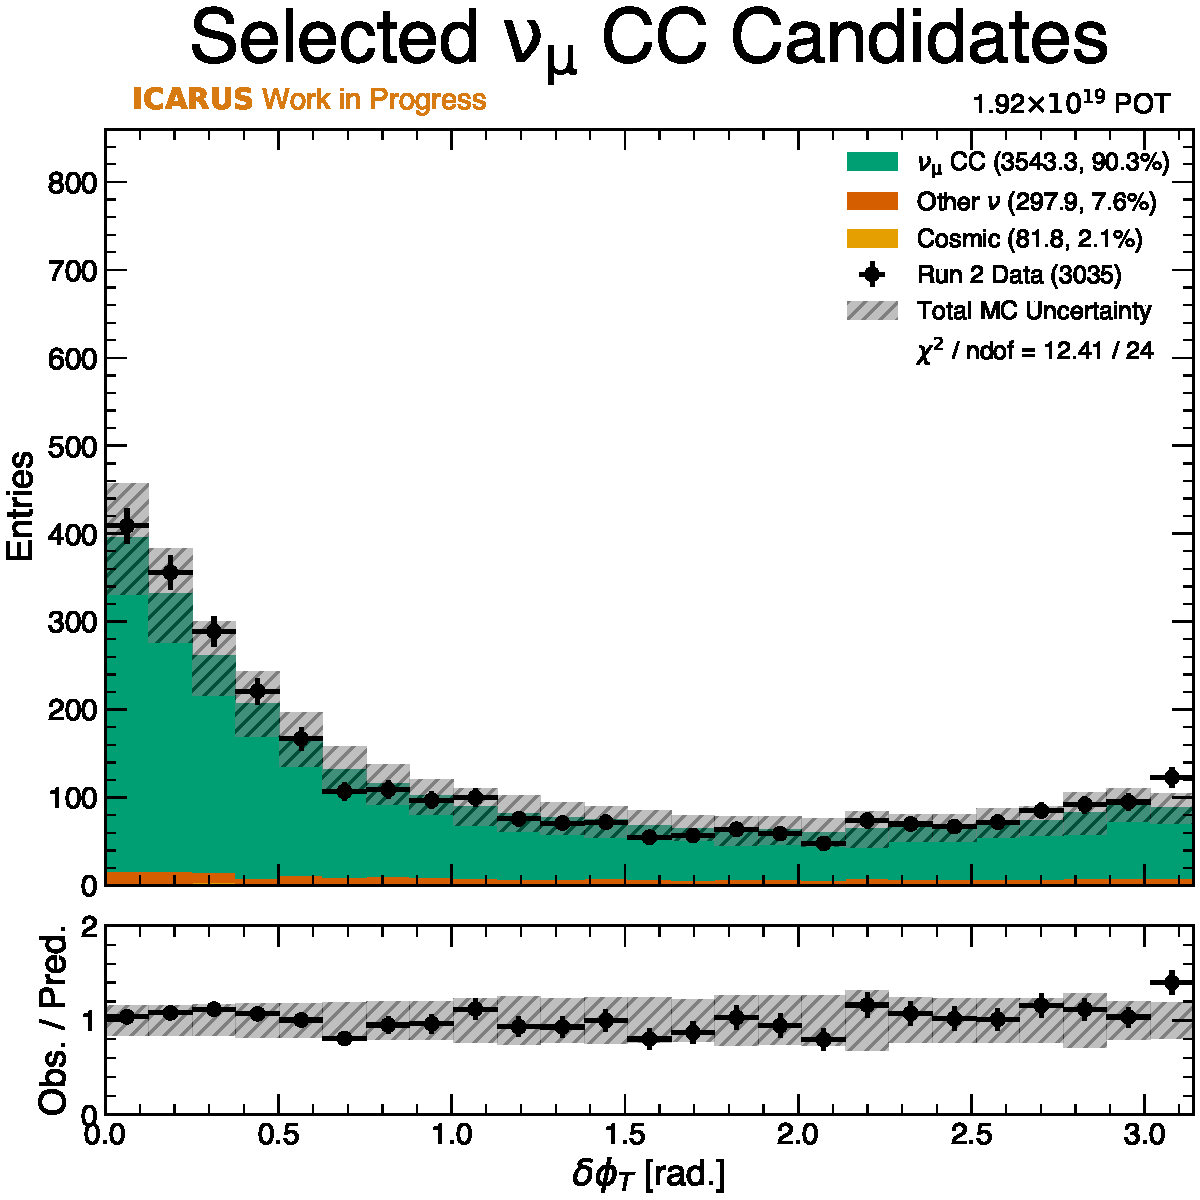
\includegraphics[width=0.42\textwidth]{figures/data_mc_comparisons/datamc_hist1d_1muX_delta_phiT.pdf}
    \caption{Comparison of data and simulation for the kinematic imbalance variables $\delta \alpha_T$ (left) and $\delta \phi_T$ (right) for each of the three signal channels: from top to bottom $\mathrm{1\mu 1p}$, $\mathrm{1\mu Np}$, and $\nu_\mu$ CC inclusive.}
    \label{fig:datamc_kinematic_imbalance_angles}
\end{figure}

The kinematic imbalance variables $\delta p_T$, $\alpha_T$, and $\phi_T$ are shown in Figures \ref{fig:datamc_delta_pT} and \ref{fig:datamc_kinematic_imbalance_angles}. These variables are commonly incorporated into cross section measurements, so it is important for any future ICARUS cross section measurements that the data and simulation do not show major biases in these variables. The discrepancy in these variables seem to be only a normalization offset, with the shape of the distributions matching well. These variables are also sensitive to smearing from poor angular reconstruction, so the agreement in these variables is a good indication that the angular reconstruction is working similarly in data and simulation.

\subsubsection{Comparisons for PID Variables}
\label{sec:datamc_pid_variables}

\begin{figure}[!htb]
    \centering
    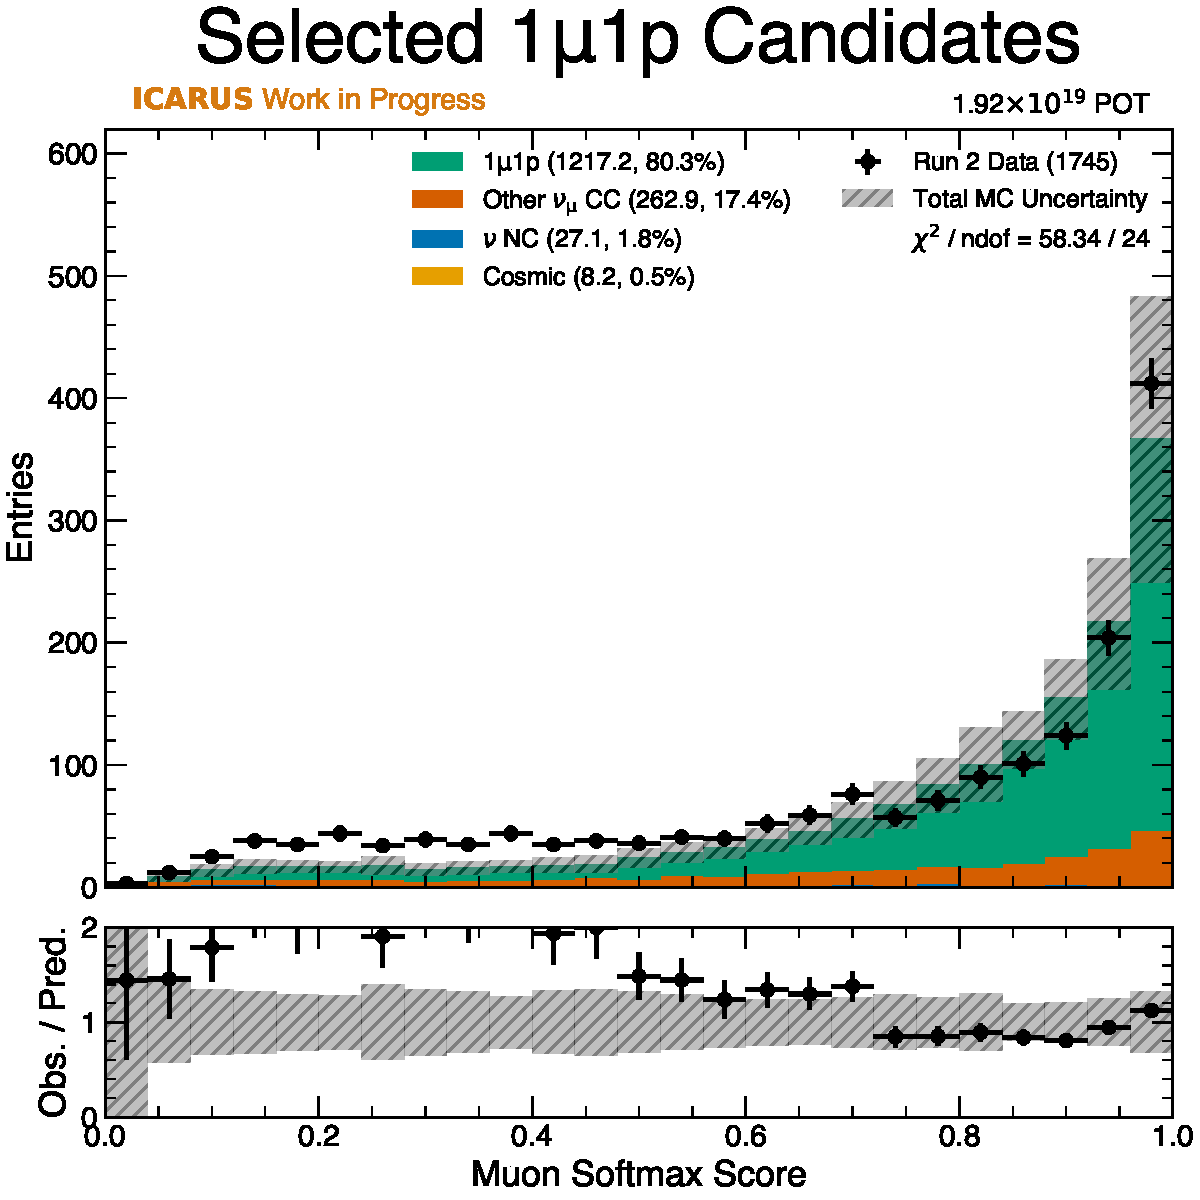
\includegraphics[width=0.42\textwidth]{figures/data_mc_comparisons/datamc_hist1d_1mu1p_muon_softmax.pdf}
    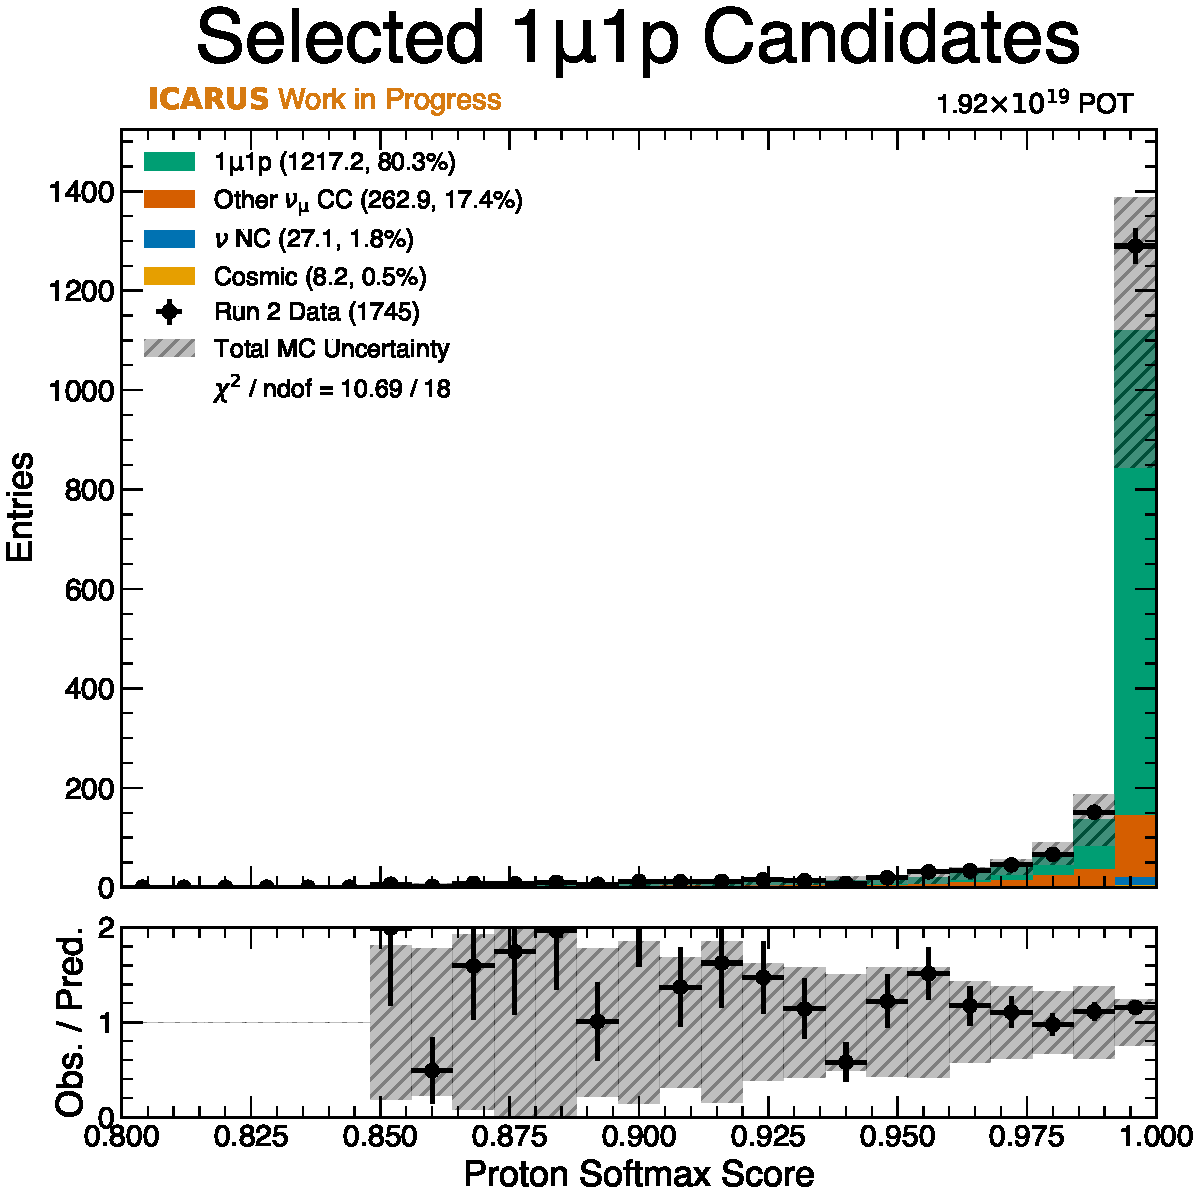
\includegraphics[width=0.42\textwidth]{figures/data_mc_comparisons/datamc_hist1d_1mu1p_proton_softmax.pdf}
    \\
    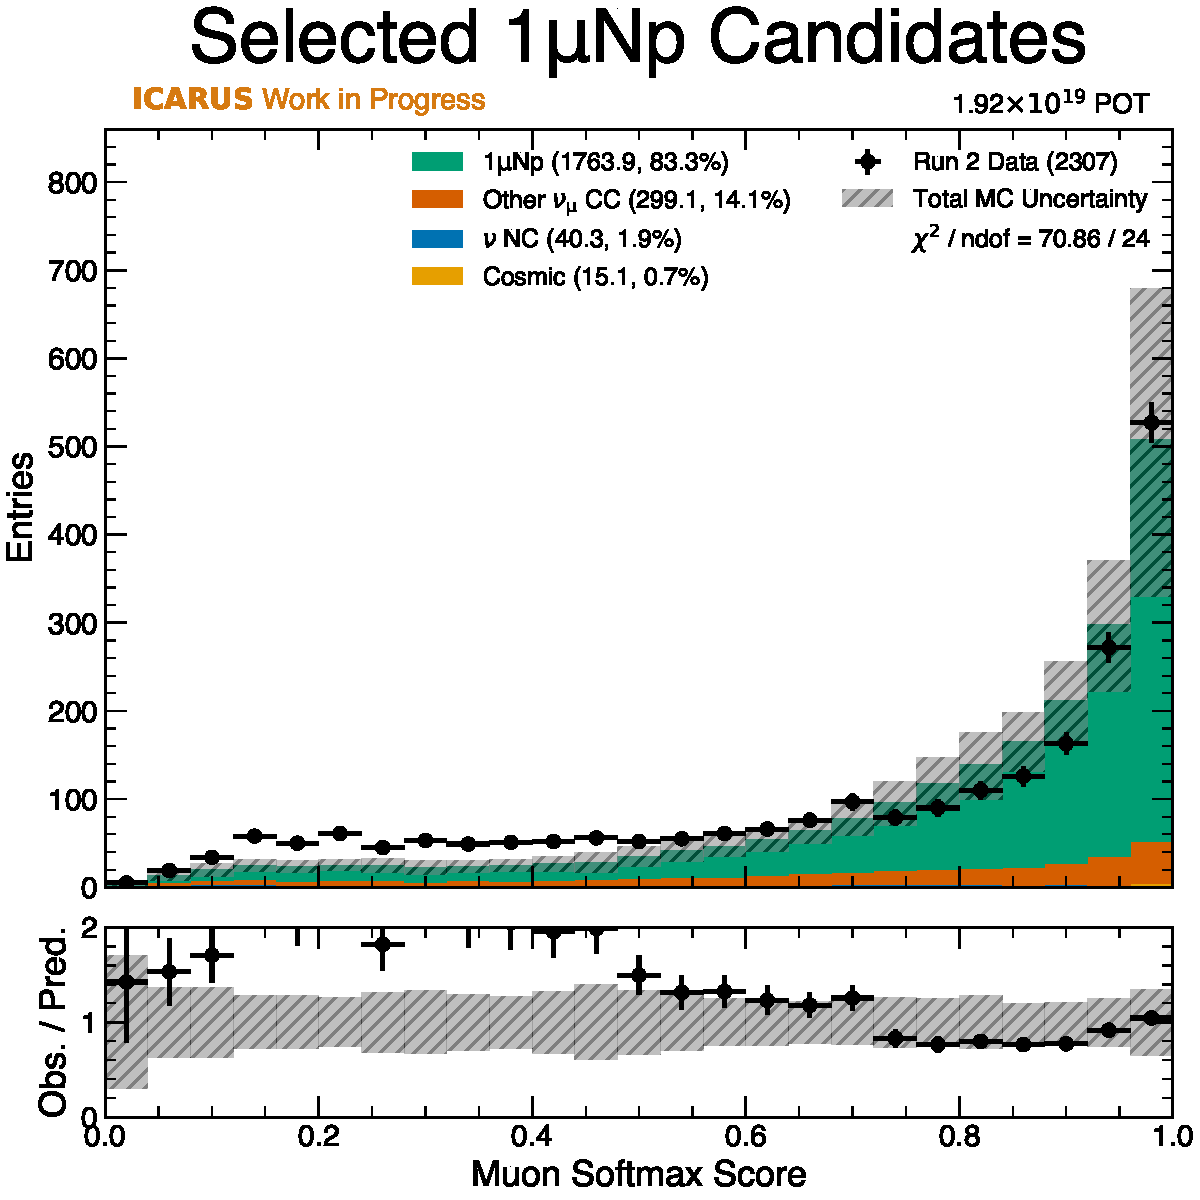
\includegraphics[width=0.42\textwidth]{figures/data_mc_comparisons/datamc_hist1d_1muNp_muon_softmax.pdf}
    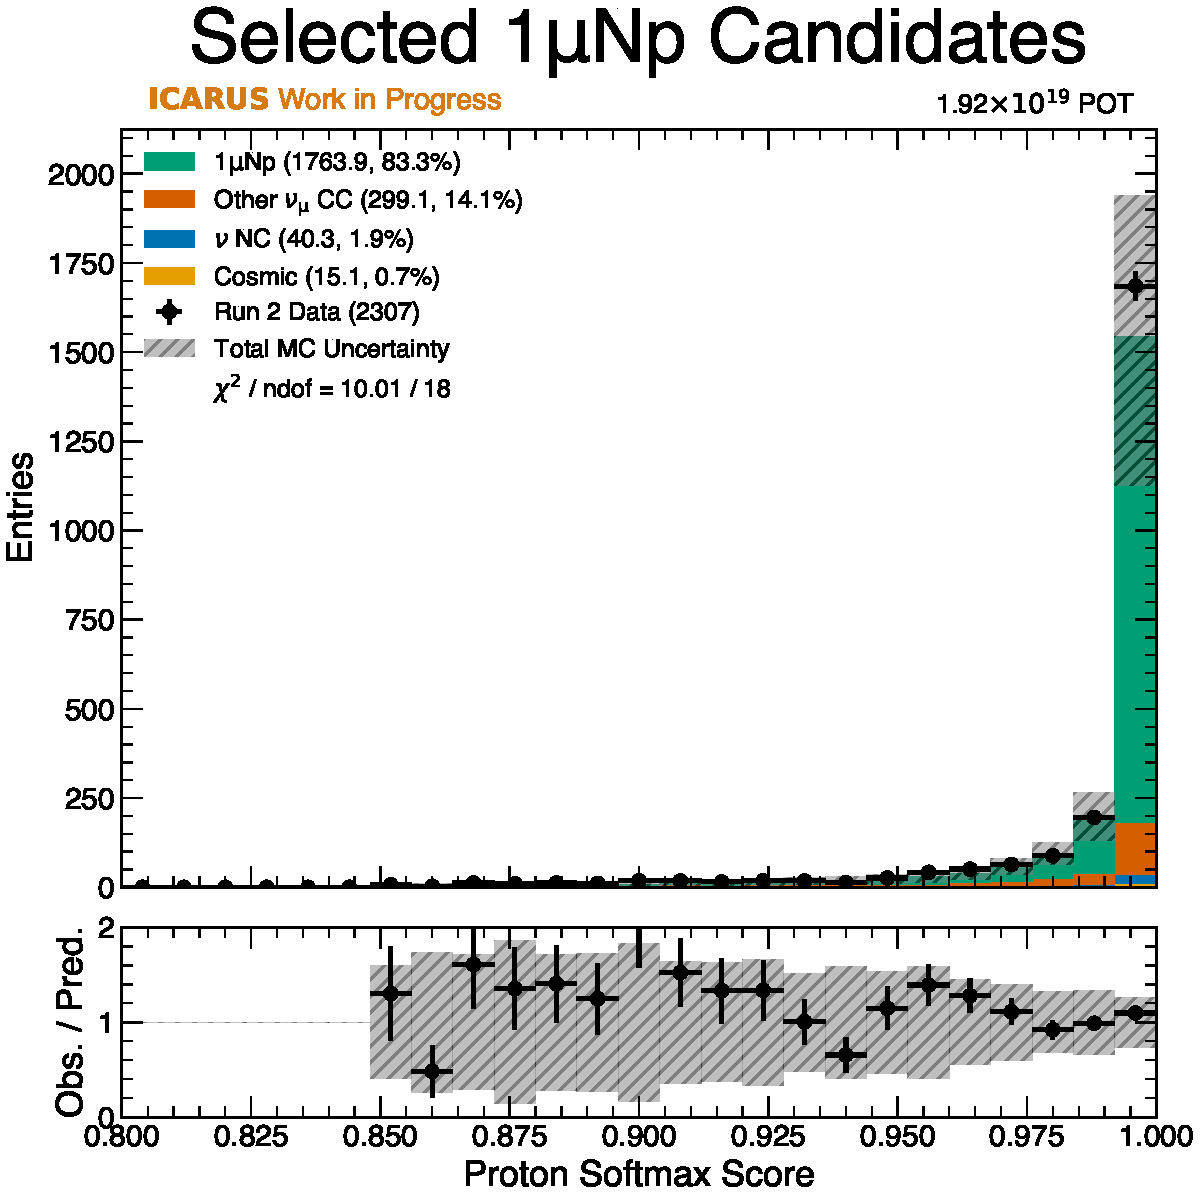
\includegraphics[width=0.42\textwidth]{figures/data_mc_comparisons/datamc_hist1d_1muNp_proton_softmax.pdf}
    \\
    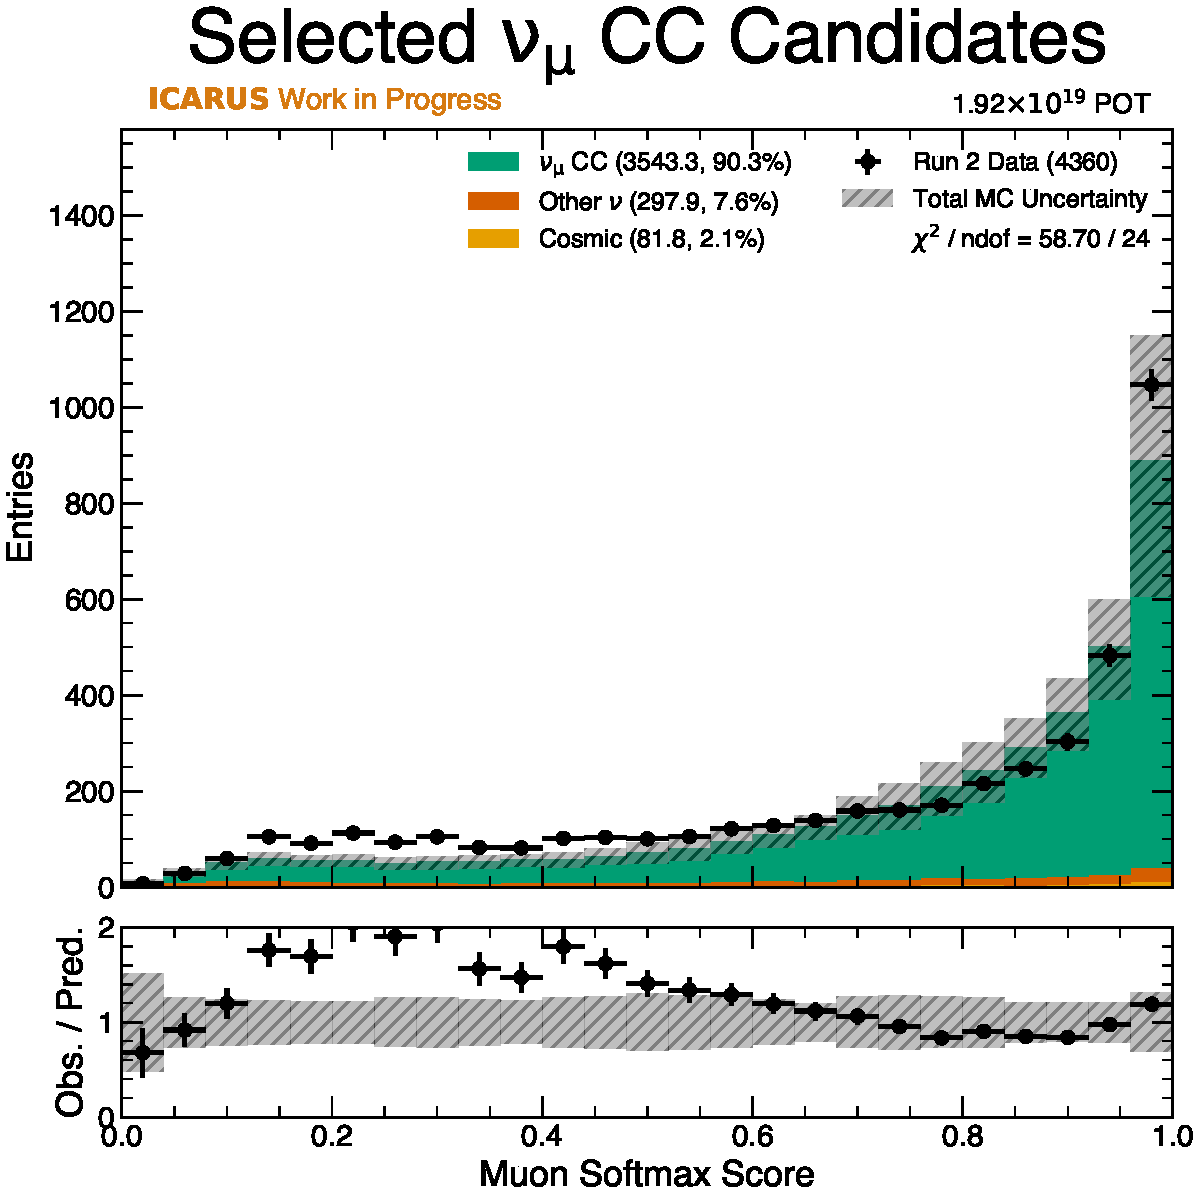
\includegraphics[width=0.42\textwidth]{figures/data_mc_comparisons/datamc_hist1d_1muX_muon_softmax.pdf}
    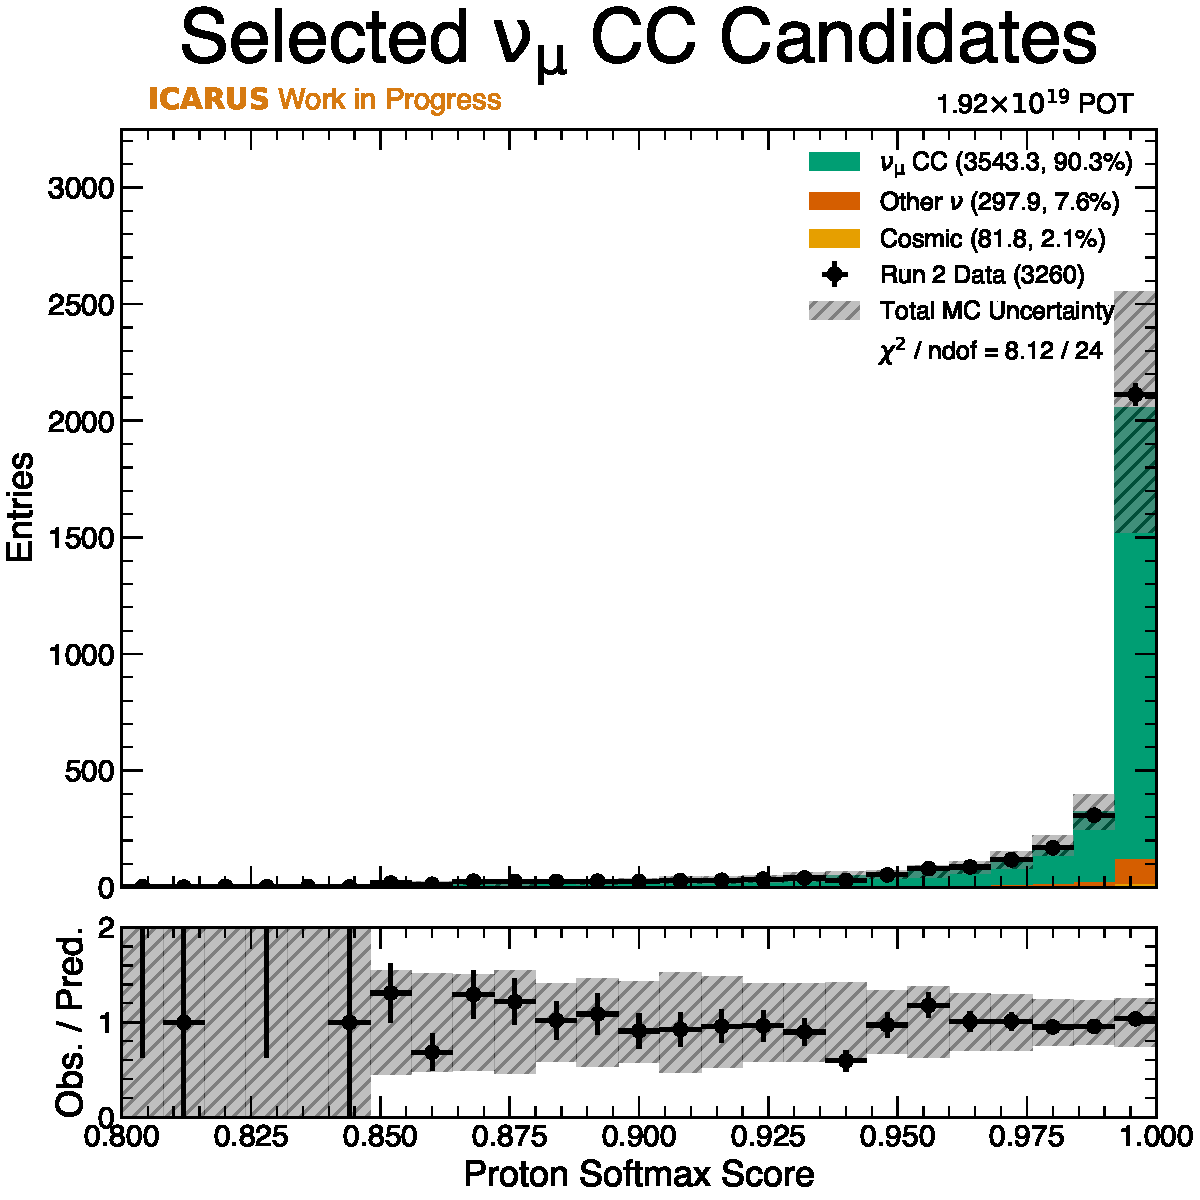
\includegraphics[width=0.42\textwidth]{figures/data_mc_comparisons/datamc_hist1d_1muX_proton_softmax.pdf}
    \caption{Comparison of data and simulation for the softmax PID scores for the muon candidate (left) and the leading proton candidate (right) for each of the three signal channels: from top to bottom $\mathrm{1\mu 1p}$, $\mathrm{1\mu Np}$, and $\nu_\mu$ CC inclusive.}
    \label{fig:datamc_softmax_pid}
\end{figure}

The PID variables are shown in Figure \ref{fig:datamc_softmax_pid}. These variables, perhaps more than any of the others, are where one would expect to see efficiency differences between data and simulation. If the PID scores are not well modeled, then it is possible that data and simulation may select interactions at different rates. There is largely good agreement in the proton PID score distributions, with only an overall normalization offset manifesting in the last bin. It is clear that the data and simulation are both confident that the leading proton candidate is a proton and to similar degrees.

The muon PID score shows a significant shift of the population from the peak to lower scores in data compared to simulation. Perhaps fortuitously, the cut placed on the muon PID score is quite low at $0.1$, so this shift does not appear to affect the selection efficiency. Regardless, this discrepancy must be understood and will be the subject of upcoming investigations. One hypothesis is that the usage of the plane-averaged charge rather than collection-only charge in the space points may be introducing a smearing effect in data that is not present in simulation. The switch to collection-only charge in the space points will require re-training the network and re-running the analysis, but it is a necessary step to understand this discrepancy. Another possible source of this discrepancy is the different value of the electron lifetime used in the Monte Carlo simulation compared to the value observed in data. This will also be the subject of future investigations.

